% === CONTEXTO === %

\vspace{2em}
\subsection{Contexto} 

Una \textit{ego-network} \cite{Leskovec} es una red compuesta por las amistades que existen entre los amigos de un individuo, el `ego'. Estas redes son centrales para aplicaciones como Facebook, Google+ o Twitter. 

En particular, dada una red `ego', resulta de interés poder identificar los circulos sociales ---conjuntos, disjuntos y anidados--- a los que pertenece un usuario. Leskovec \cite{Leskovec} propone un método de aprendizaje no supervisado para lograr inferirlos, que se nutre de la siguiente información: un grafo \textbf{E} (la red) ---donde se espera que exista una correlación fuerte entre un círculo y la densidad de conexiones entre los nodos que lo componen--- y un conjunto de atributos \textbf{C}, para cada nodo ---donde se espera una correlación entre un círculo y la similaridad de los atributos de los nodos que lo componen---.

\vspace{1em}
En este análisis estimaremos \textbf{E}, una red `ego' proveniente de Facebook, por medio de la construcción de una matriz de similaridad que utilice los atributos definidos en \textbf{C}. También, buscaremos reducir su dimensionalidad por medio del análisis de componentes principales.

% === SIMILARIDAD @ ATRIBUTOS === %

\vspace{2em}
\subsection{Matriz de similaridad}

Queremos generar una aproximación de nuestra red `ego' original \textbf{E} en base a los atributos en \textbf{C} de los usuarios que la componen. Es decir, buscamos un método que nos permita comparar los atributos de dos nodos diferentes y, bajo algún criterio propuesto, conectarlos o no en fin de replicar nuestra red verdadera. 

Intuitivamente, una forma de adivinar si dos usuarios se encuentran conectados en una red es contando la cantidad de atributos que comparten. Se podría pensar que si coinciden en muchos existe una mayor probabilidad de que pertenezcan al mismo círculo, mientras que sino podría ser que ni siquiera se conozcan. Las estructuras que utilizaremos para replicar esta línea de pensamiento son las \textit{matrices de similaridad}, las cuales dado un conjunto de datos $X$ aplican una función a cada par de datos $ij$.

\begin{equation}
    S_{ij} = f(X_i, X_j)
\end{equation}

Nuestra tabla de atributos\footnote{La misma puede encontrarse en \textit{./catedra/ego-facebook.feat}.} es tal que la primera columna contiene los tags correspondientes a cada usuario, y el resto de las columnas forman \textbf{C}, donde la $fila_i(\textbf{C})$ son los atributos del usuario $tag_i$. Tomemos entonces nuestra matriz de similaridad $\textbf{S} = \textbf{CC}^{t}$, tal que $\textbf{S}_{ij}$ expresa la similaridad entre la $tag_{i}$ y $tag_{j}$ computando el producto interno de sus respectivos atributos. Con esta información podemos luego proponer diferentes umbrales $u$ entre el menor y mayor valor en \textbf{S}, y establecer que $\textbf{S}_{ij} > u$ indica que los $tag_{i}$ y $tag_{j}$ están conectados en nuestra aproximación. 

Procedemos a mostrar los resultados obtenidos. Tomando $u \in [min{\textbf{S}_{ij}},\ max{\textbf{S}_{ij}}) = [0, 22)$, $u \in \mathbb{Z}$, obtuvimos 22 diferentes aproximaciones de \textbf{E}.
Obsérvese que cuanto más alto sea el umbral, menores conexiones tendremos en nuestro grafo aproximado. En particular, con $u = 0$ se obtiene un grafo donde todos los usuarios están conectados entre sí, y con $u > 12$ grafos con ninguna arista. Nos enfocaremos entonces con los asociados a $u \in [0, 12]$, ya que son los que revelan información de interés.

\vspace{1em}

\begin{figure}[!htbp]
    \centering
    \subfloat[Original]{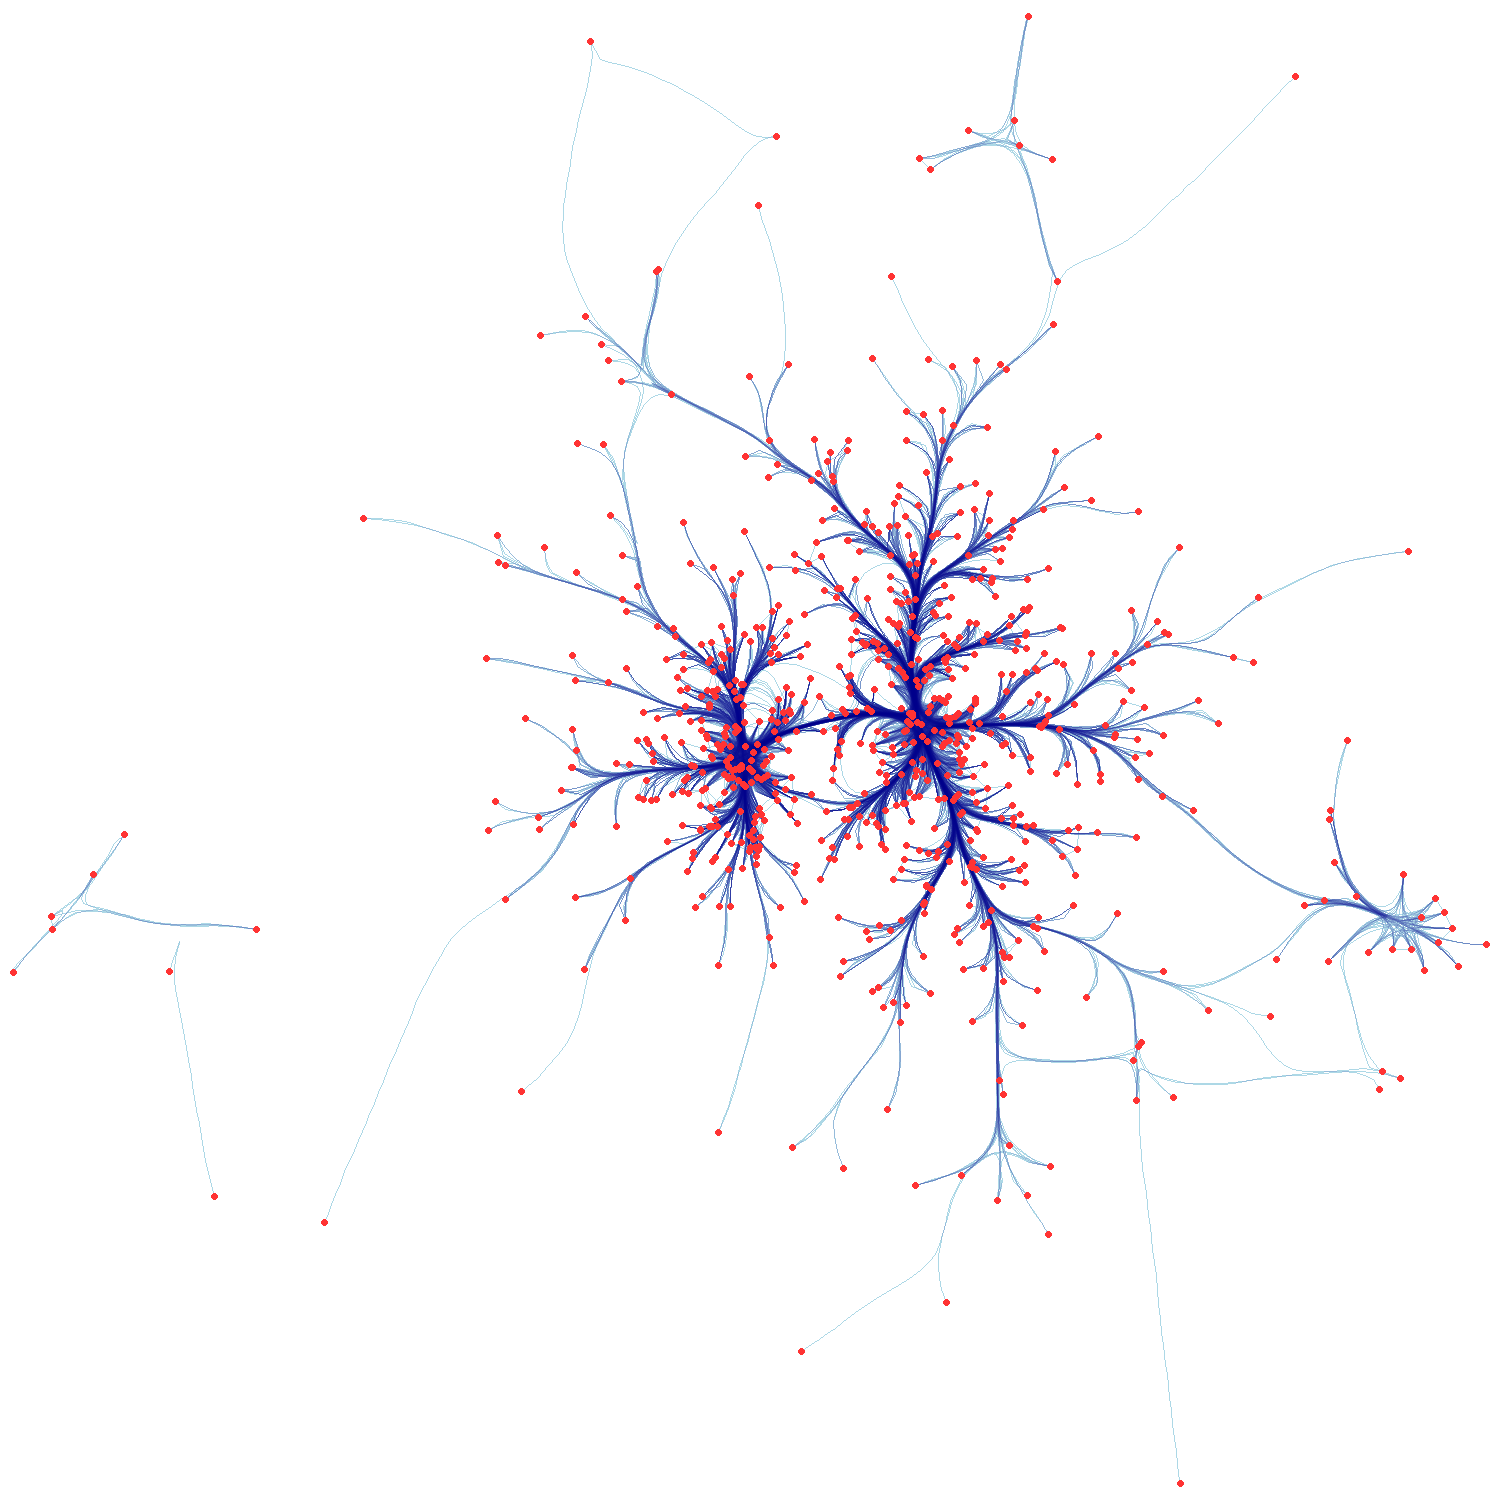
\includegraphics[width=.25\textwidth]{/files/src/.media/ego/grafo_forceatlas2_facebook.png}}\hfill
    \subfloat[$u = 0$]{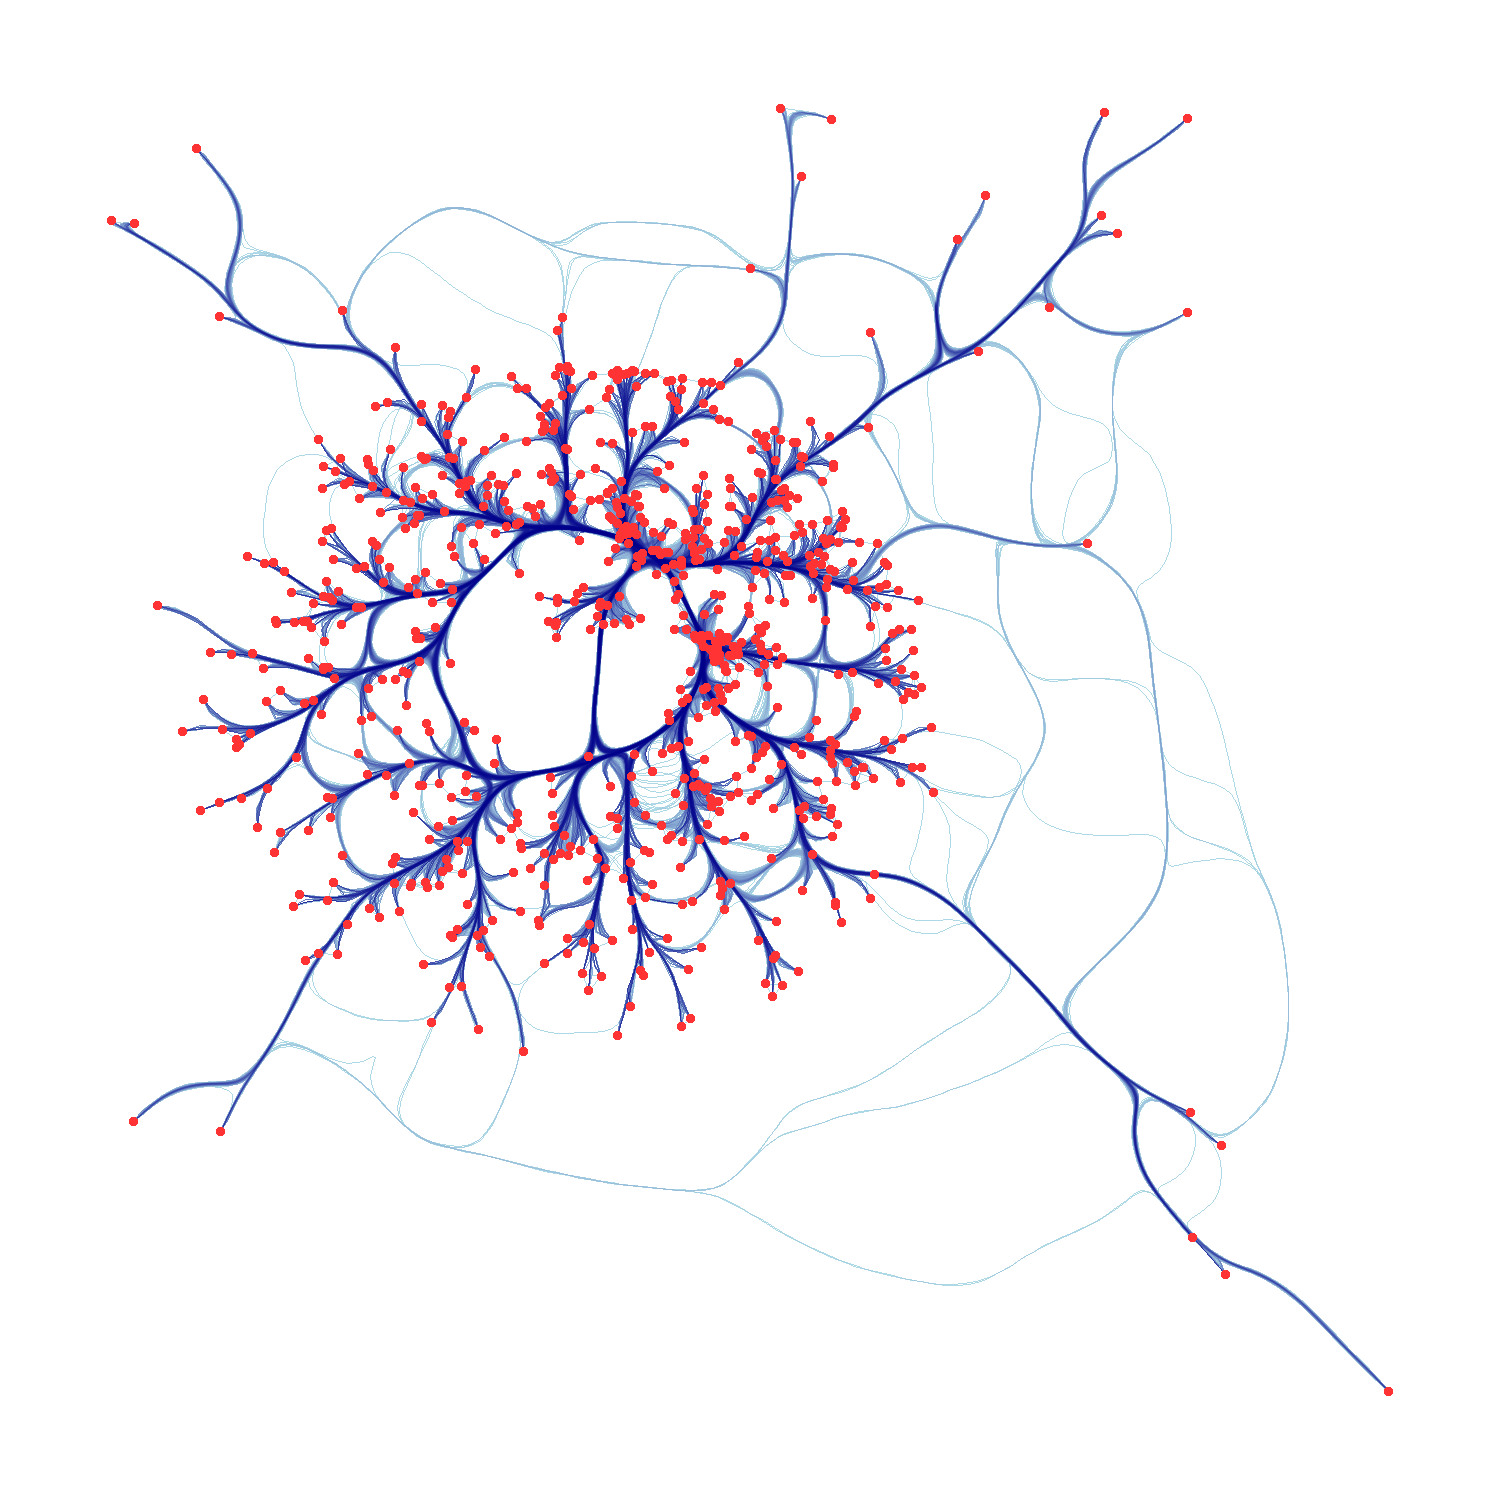
\includegraphics[width=.25\textwidth]{/files/src/.media/ego/grafo_forceatlas2_0.png}}\hfill
    \subfloat[$u = 1$]{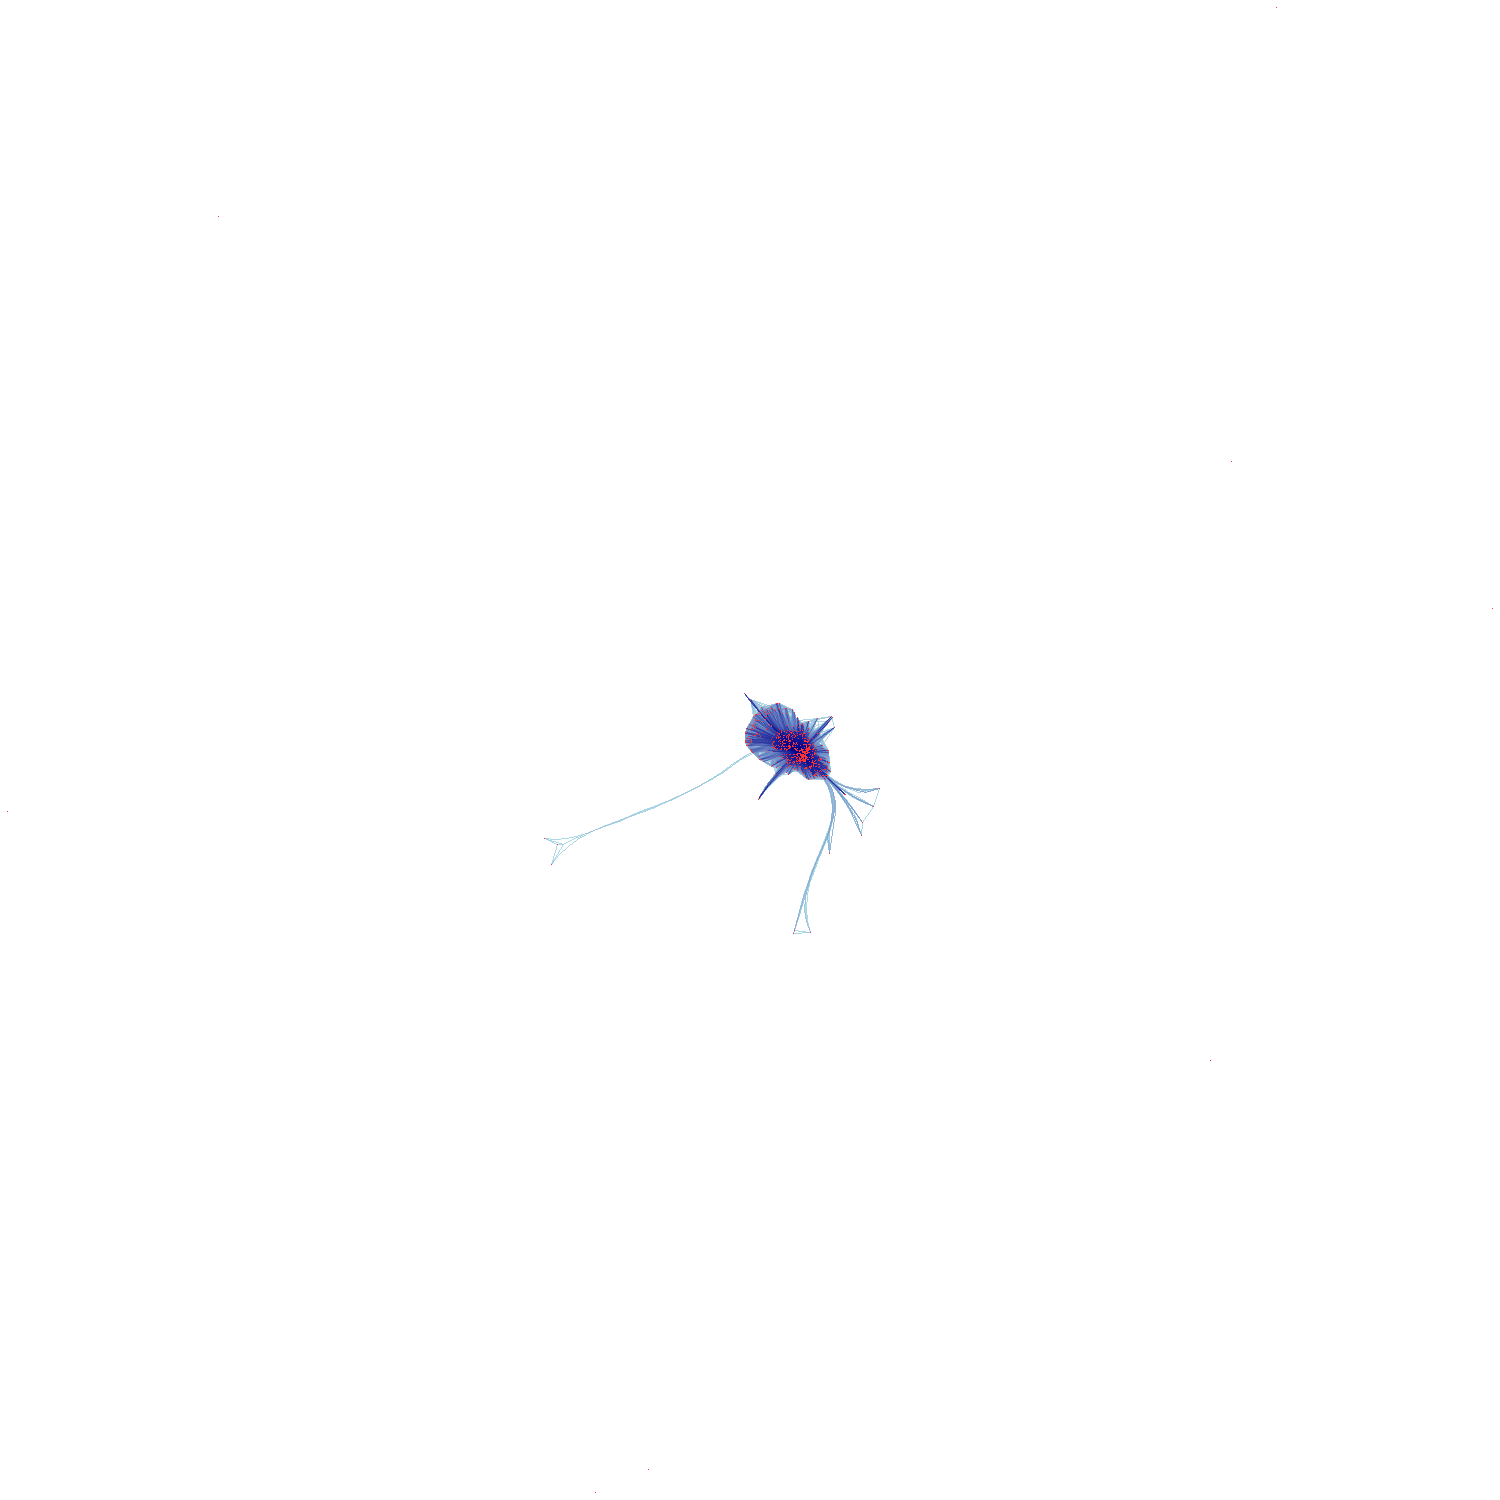
\includegraphics[width=.25\textwidth]{/files/src/.media/ego/grafo_forceatlas2_1.png}}\hfill
    \subfloat[$u = 2$]{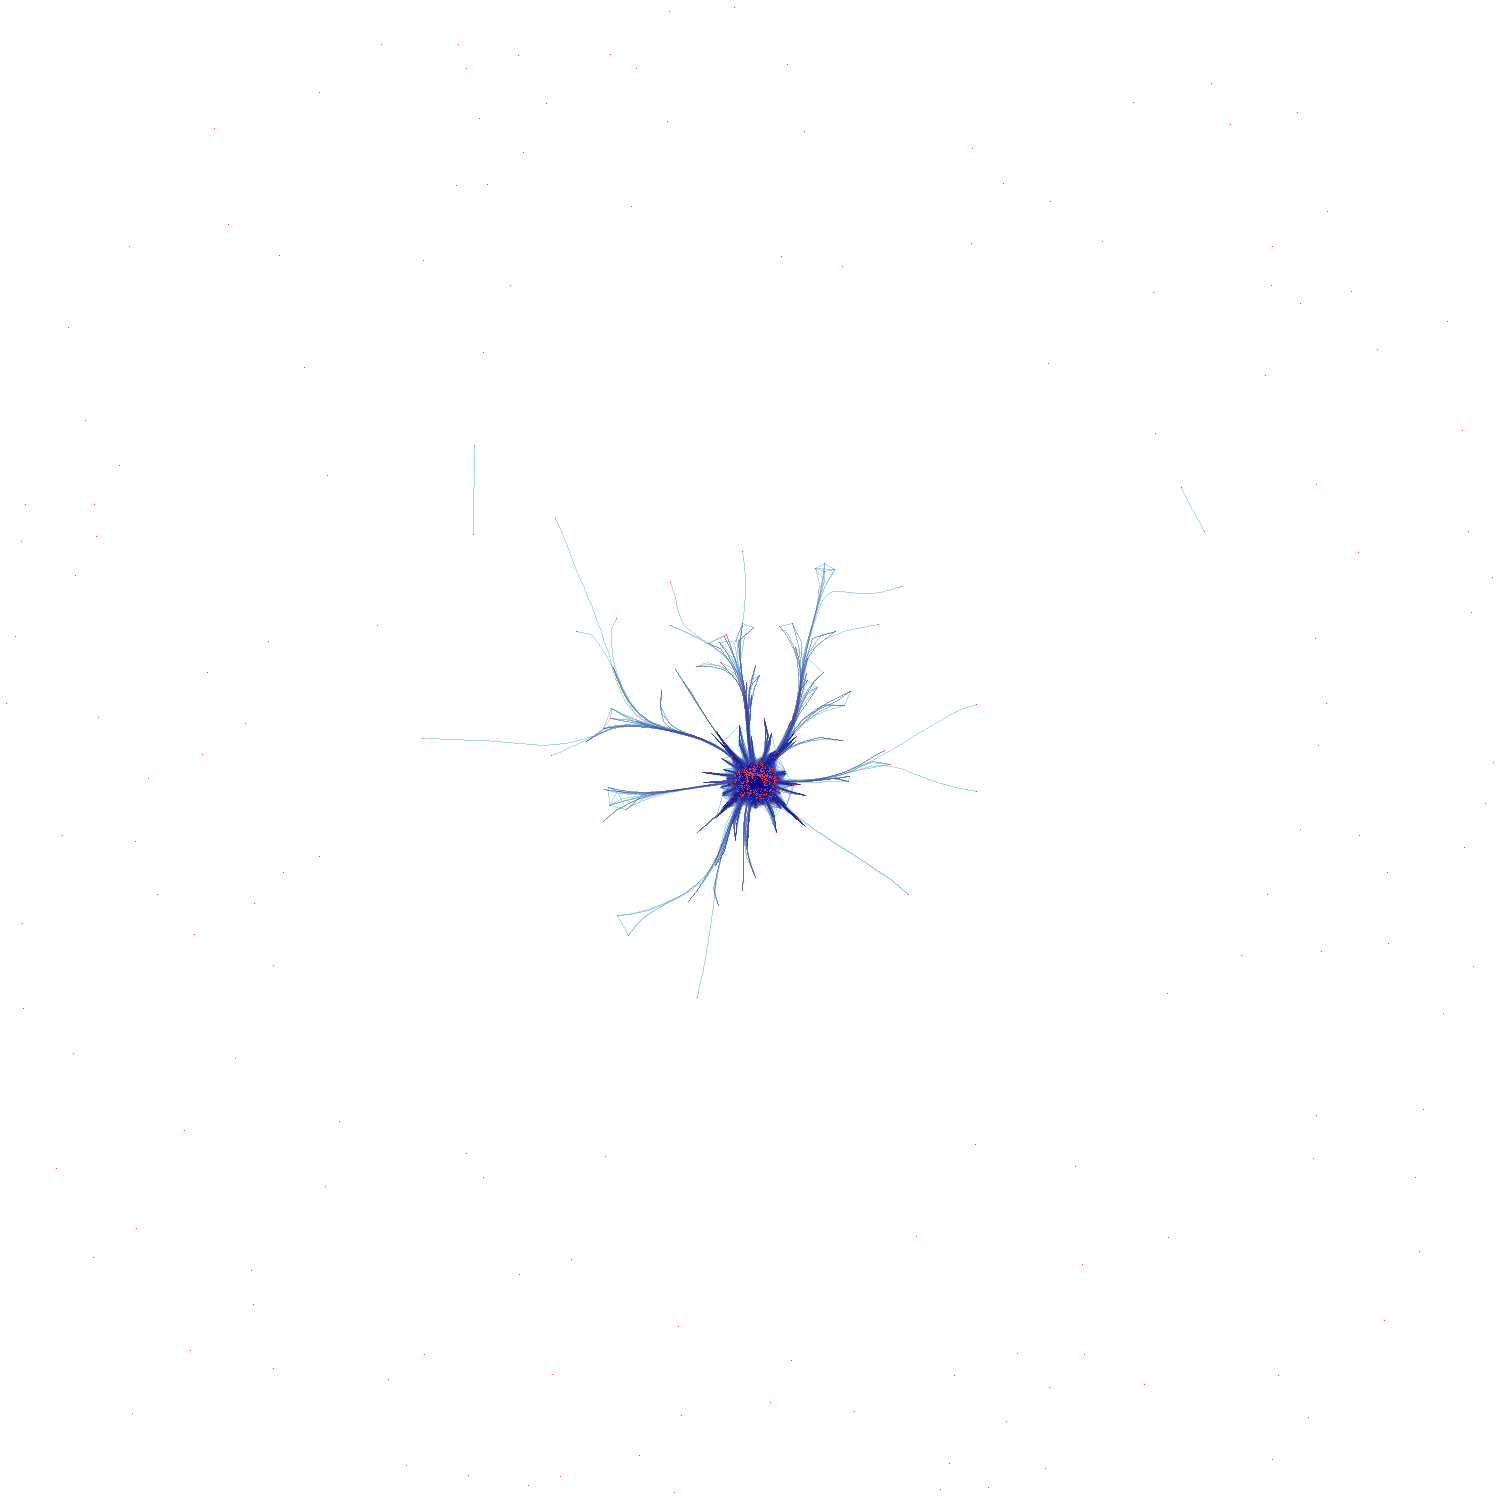
\includegraphics[width=.25\textwidth]{/files/src/.media/ego/grafo_forceatlas2_2.png}}\hfill
    \\[\smallskipamount]
    \subfloat[$u = 3$]{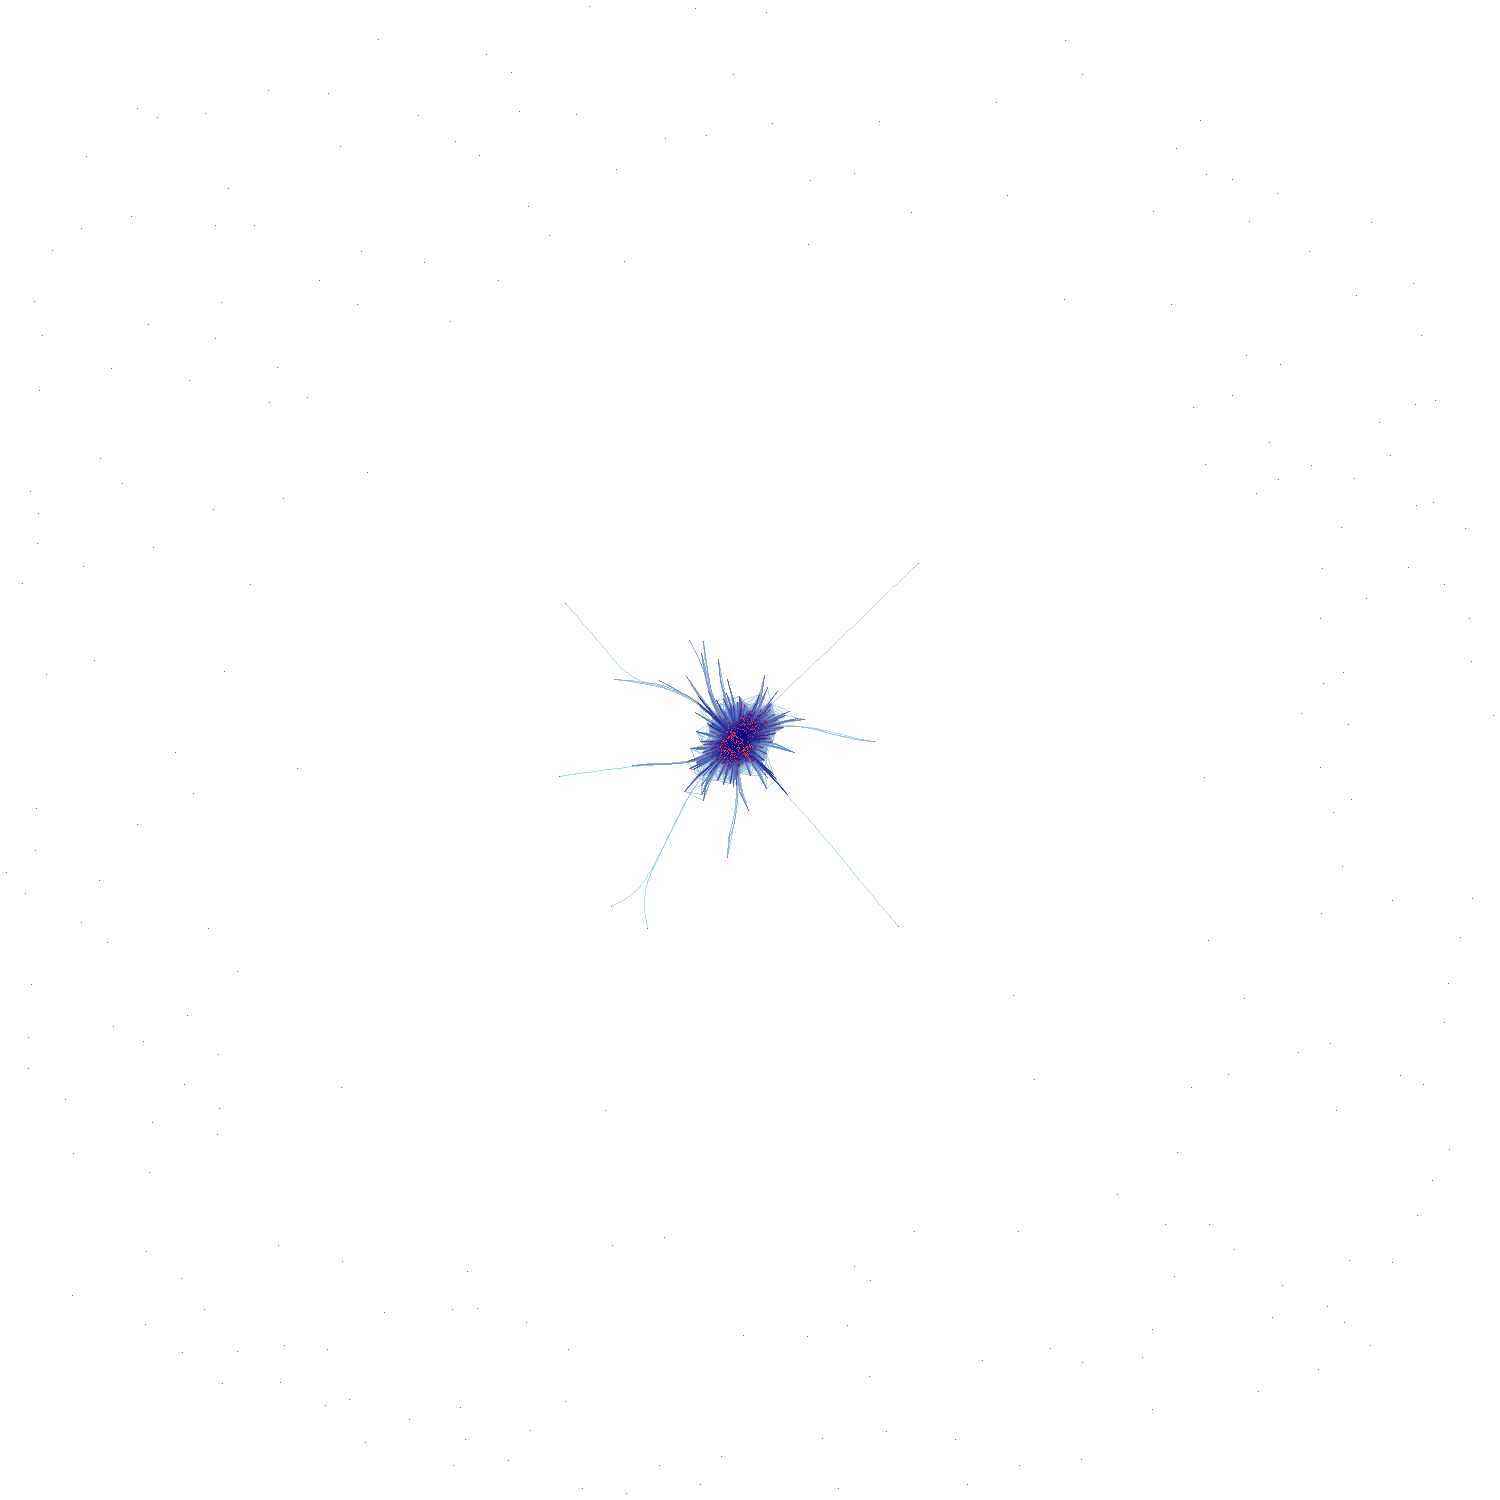
\includegraphics[width=.25\textwidth]{/files/src/.media/ego/grafo_forceatlas2_3.png}}\hfill
    \subfloat[$u = 4$]{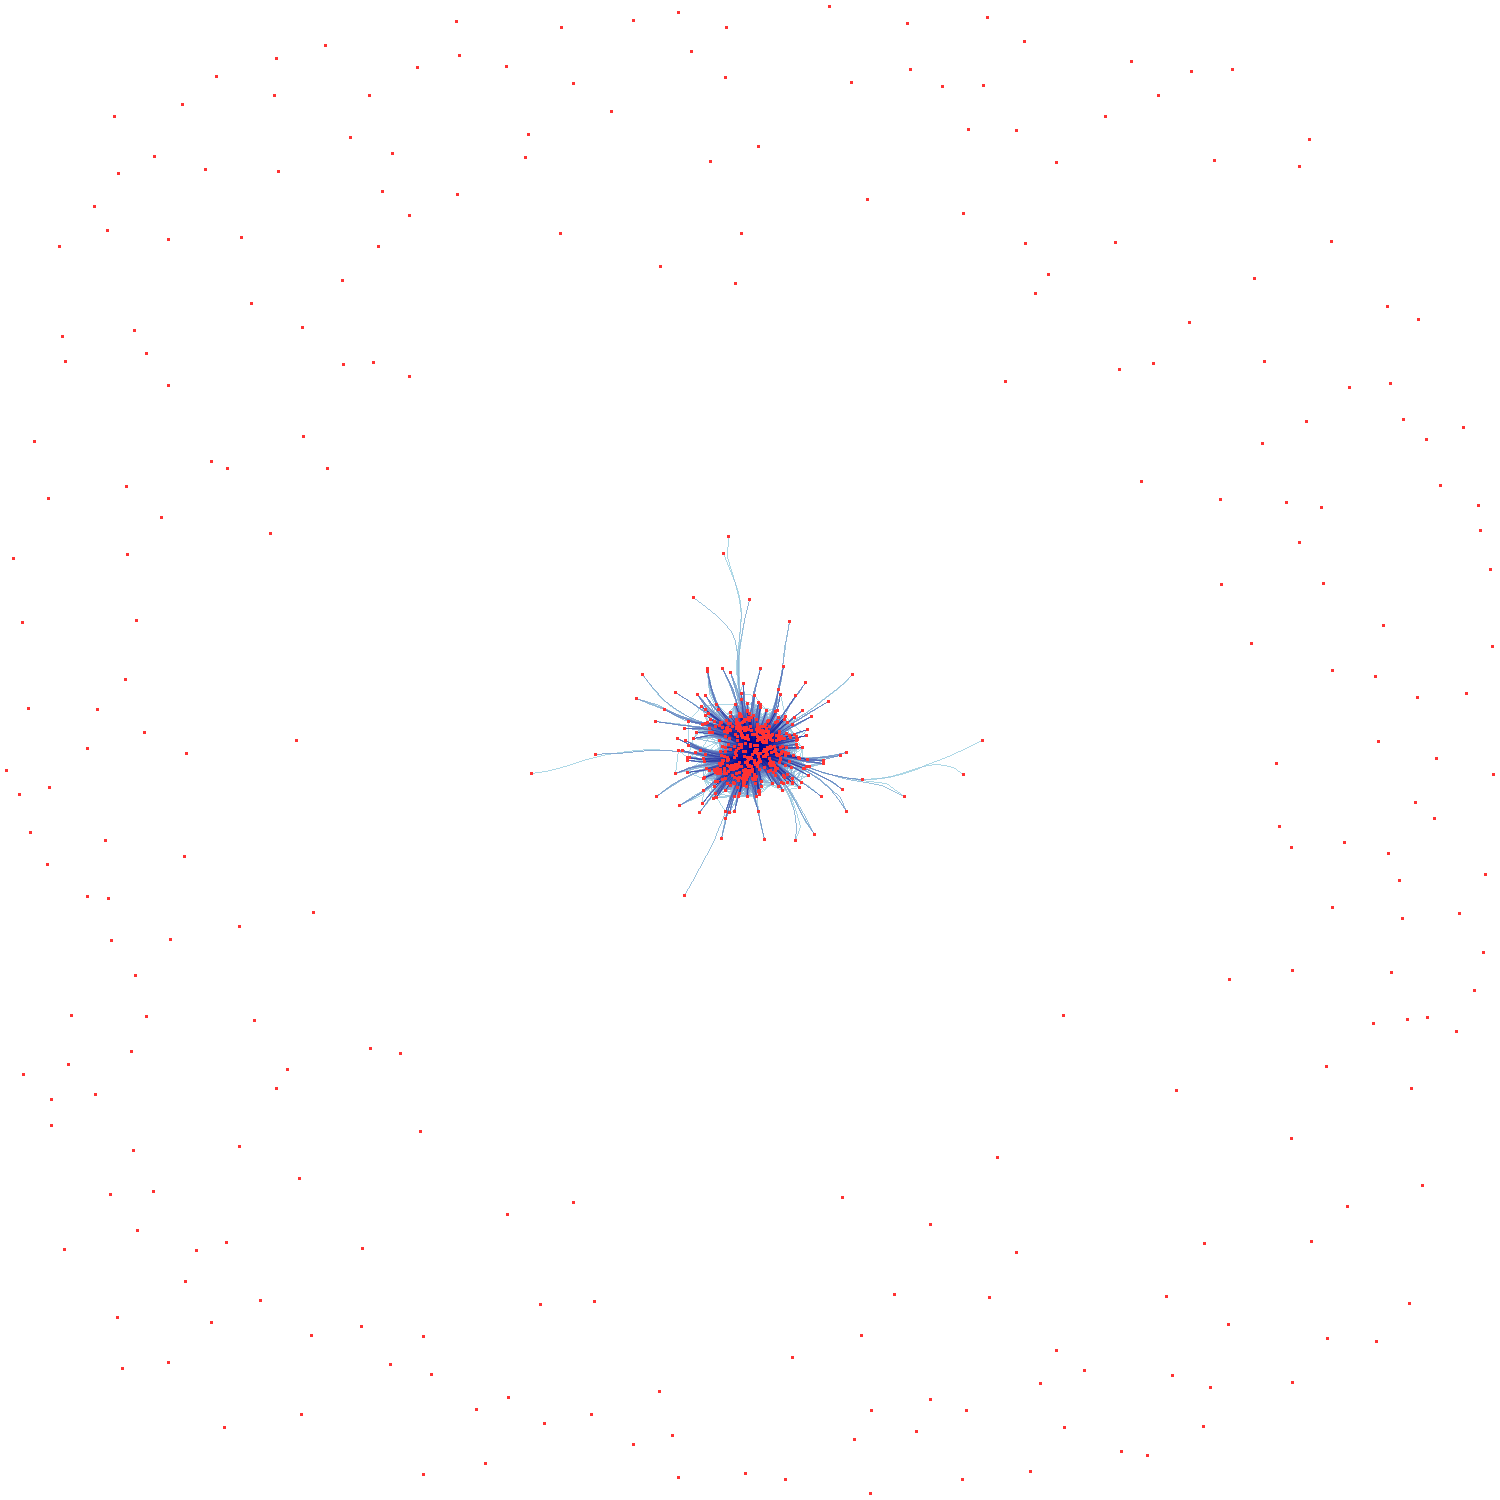
\includegraphics[width=.25\textwidth]{/files/src/.media/ego/grafo_forceatlas2_4.png}}\hfill
    \subfloat[$u = 5$]{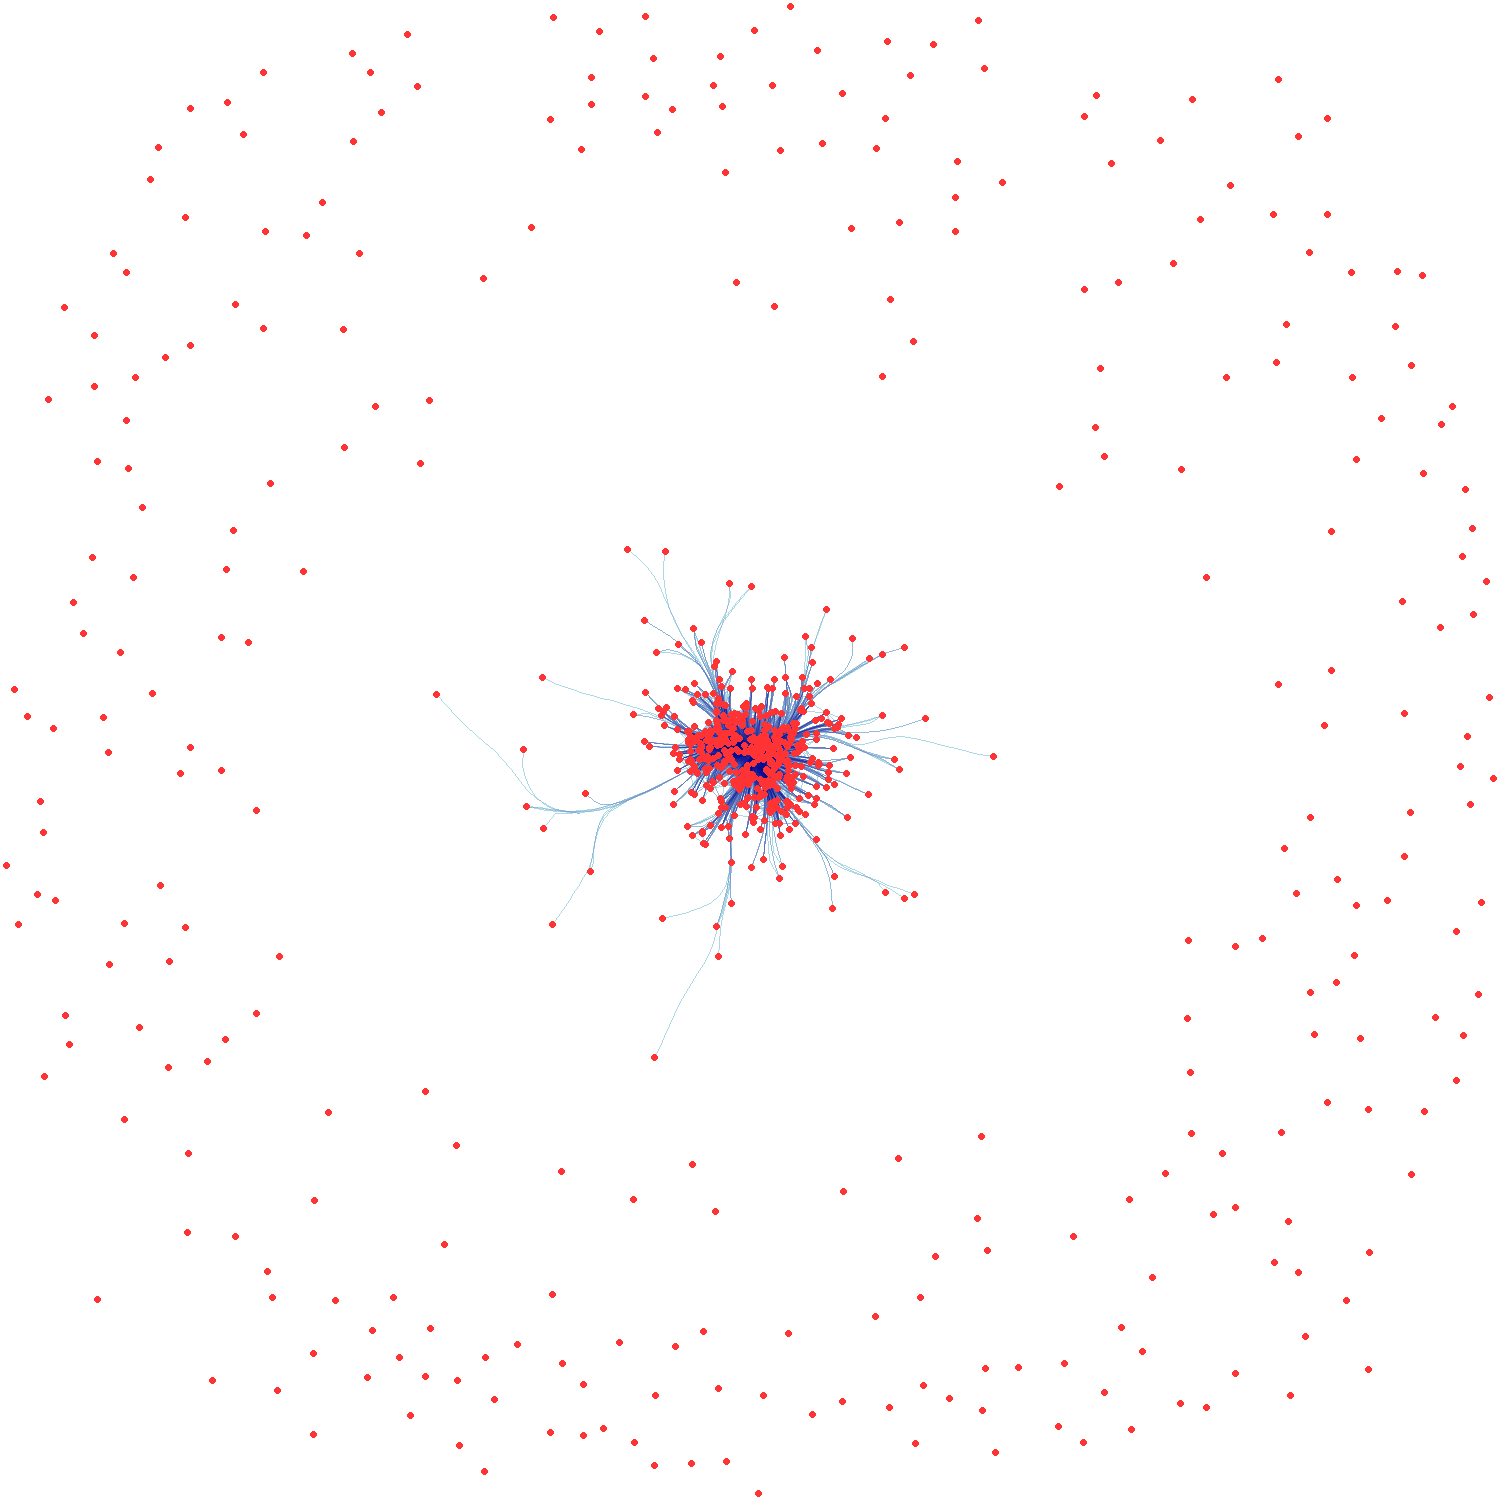
\includegraphics[width=.25\textwidth]{/files/src/.media/ego/grafo_forceatlas2_5.png}}\hfill
    \subfloat[$u = 6$]{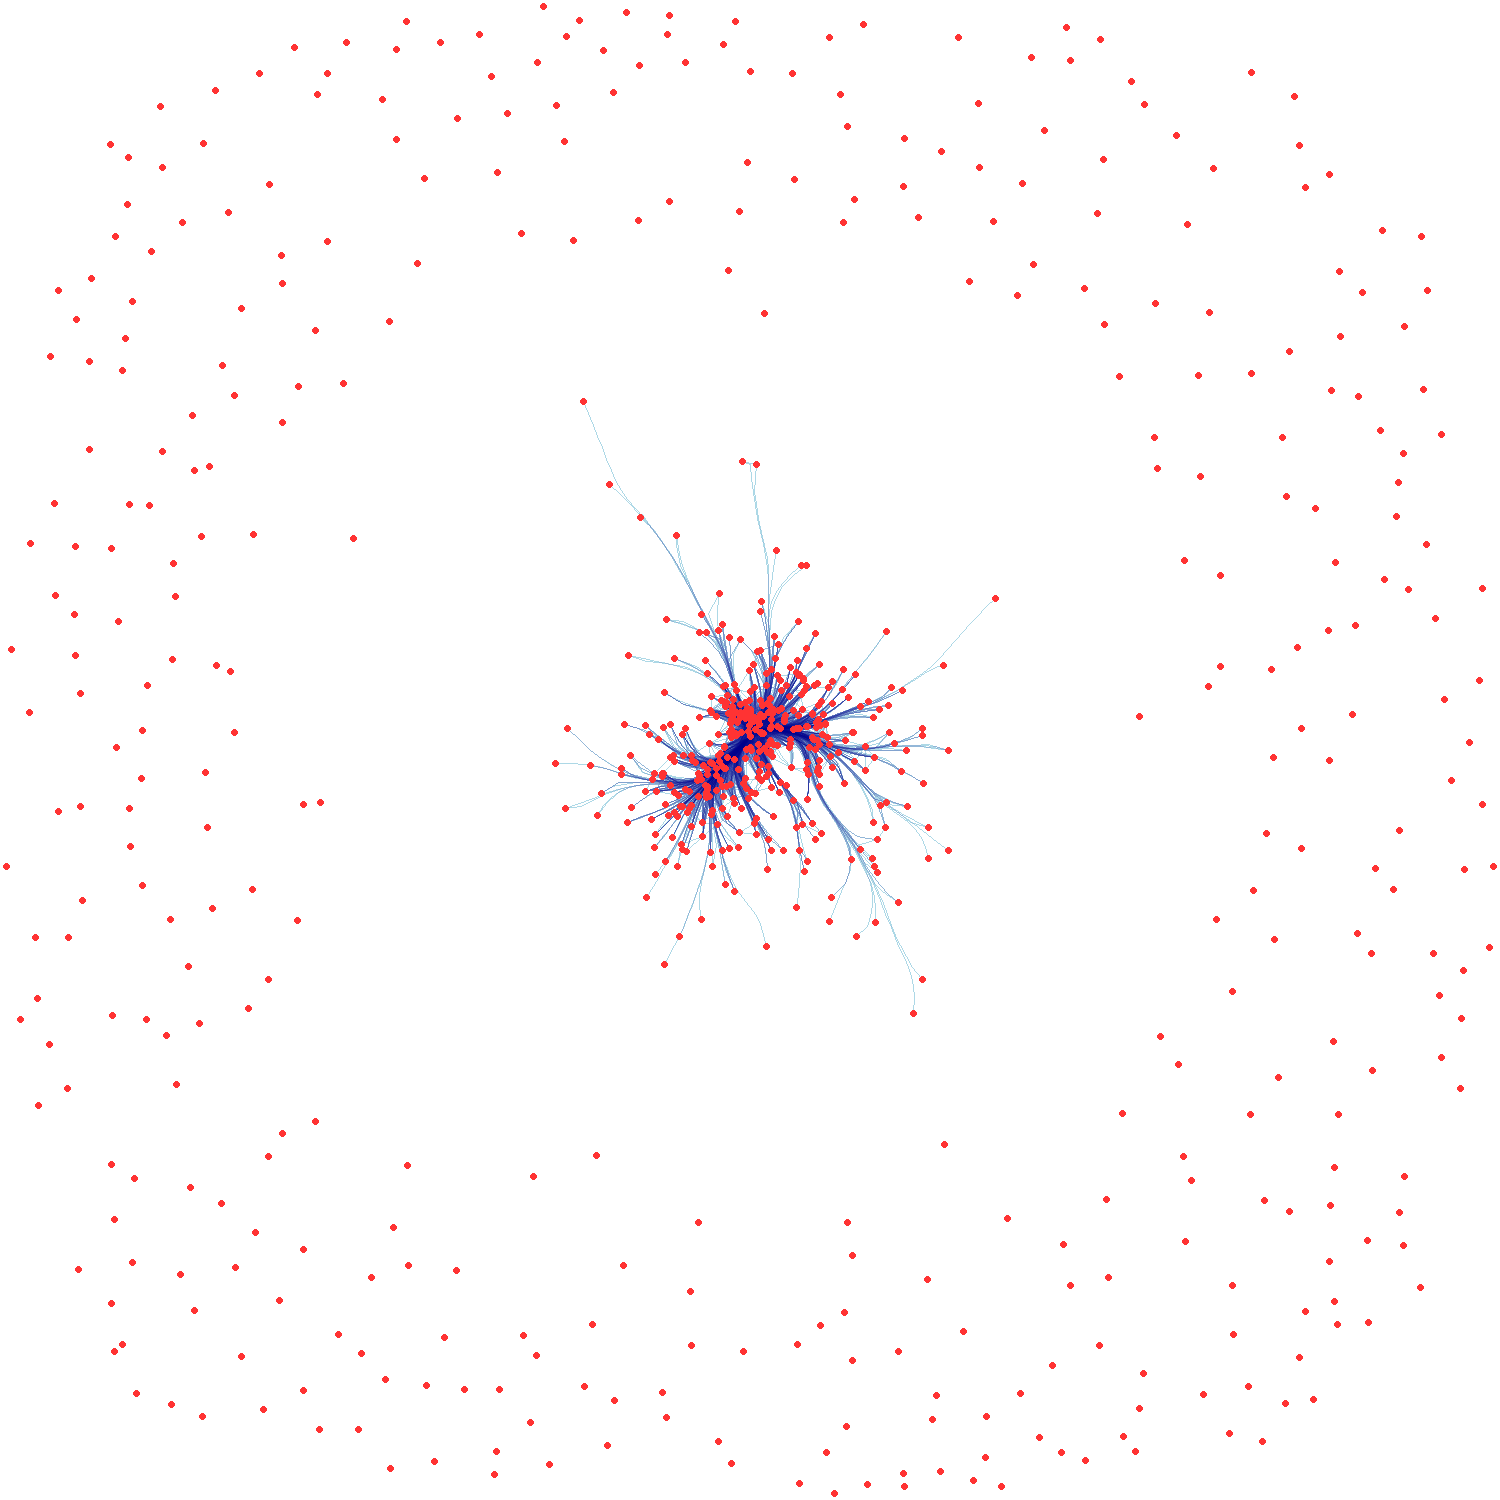
\includegraphics[width=.25\textwidth]{/files/src/.media/ego/grafo_forceatlas2_6.png}}\hfill
    \\[\smallskipamount]
    \subfloat[$u = 7$]{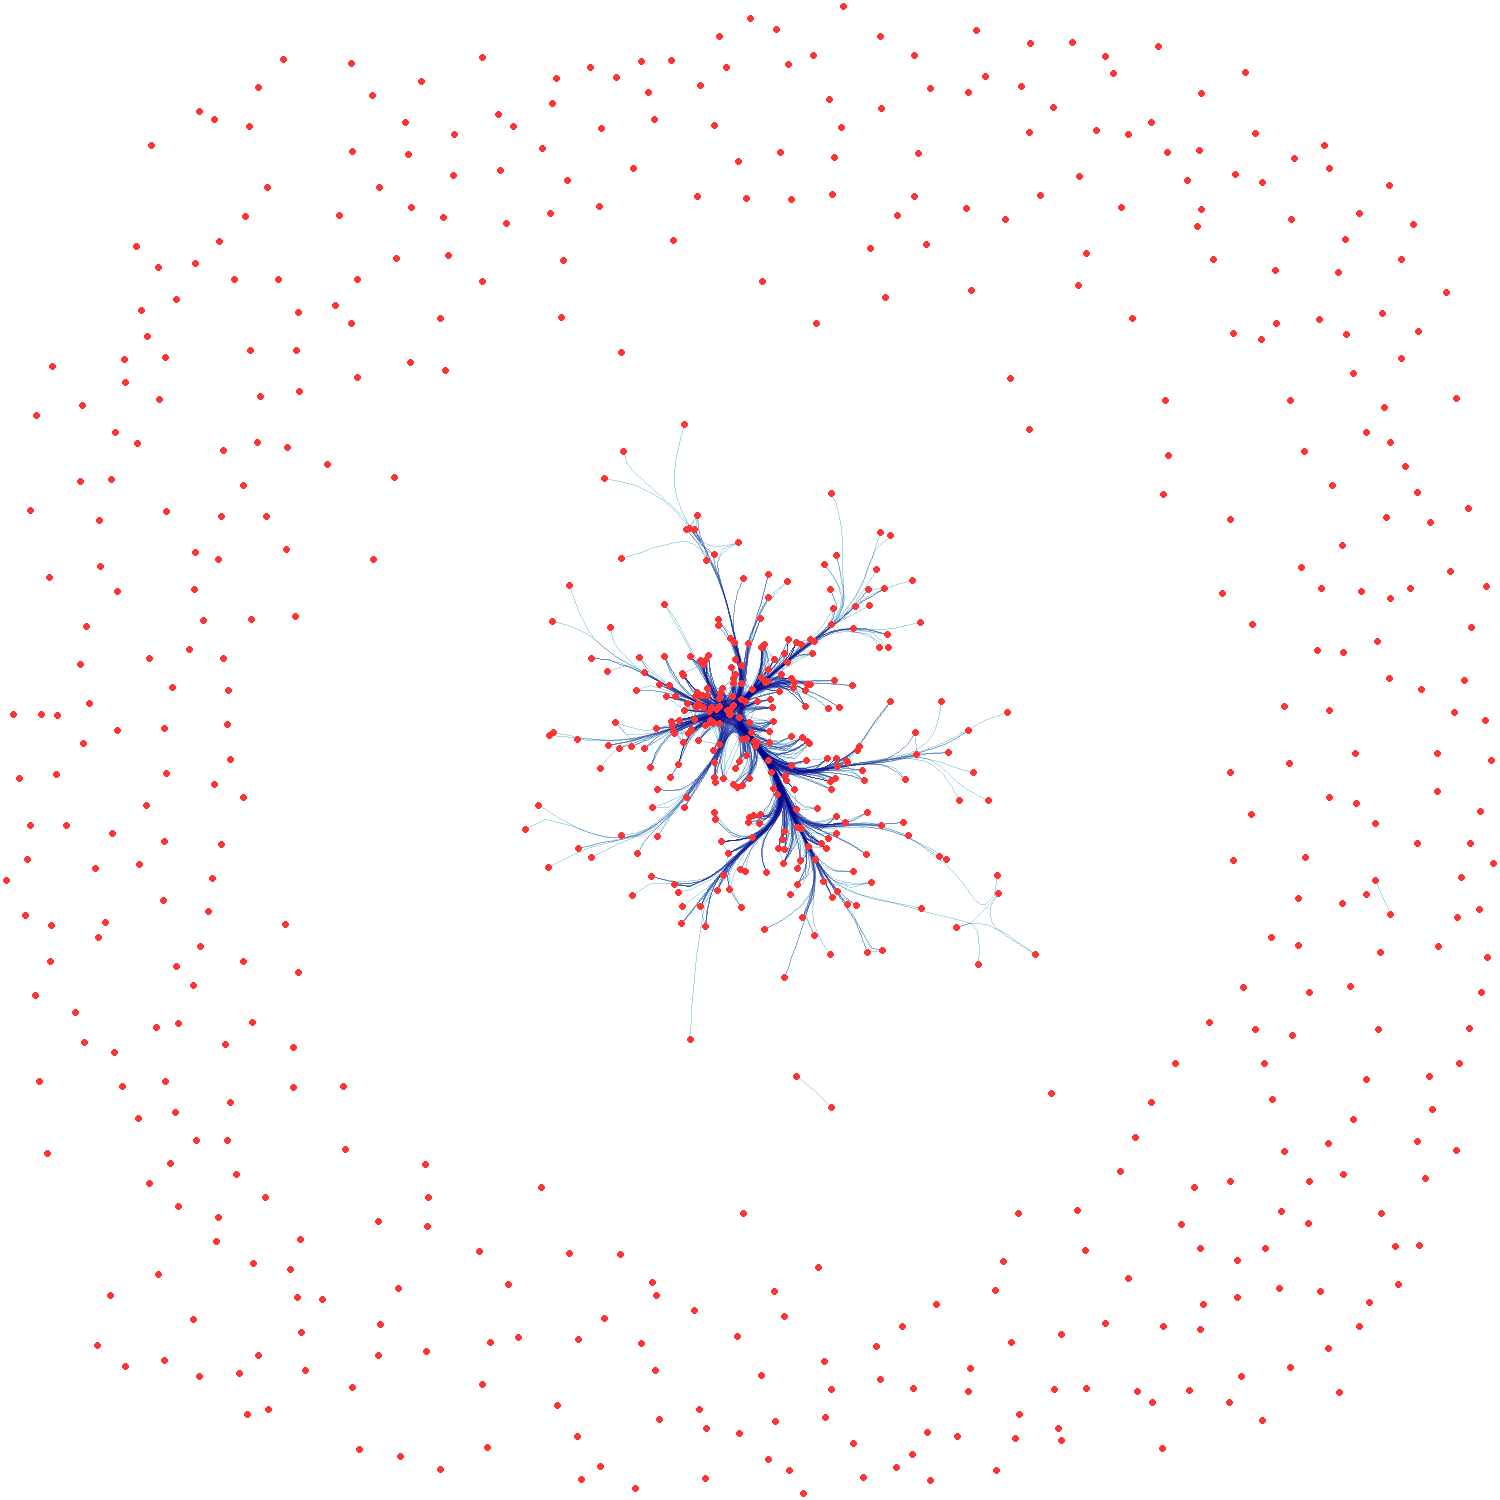
\includegraphics[width=.25\textwidth]{/files/src/.media/ego/grafo_forceatlas2_7.png}}\hfill    
    \subfloat[$u = 8$]{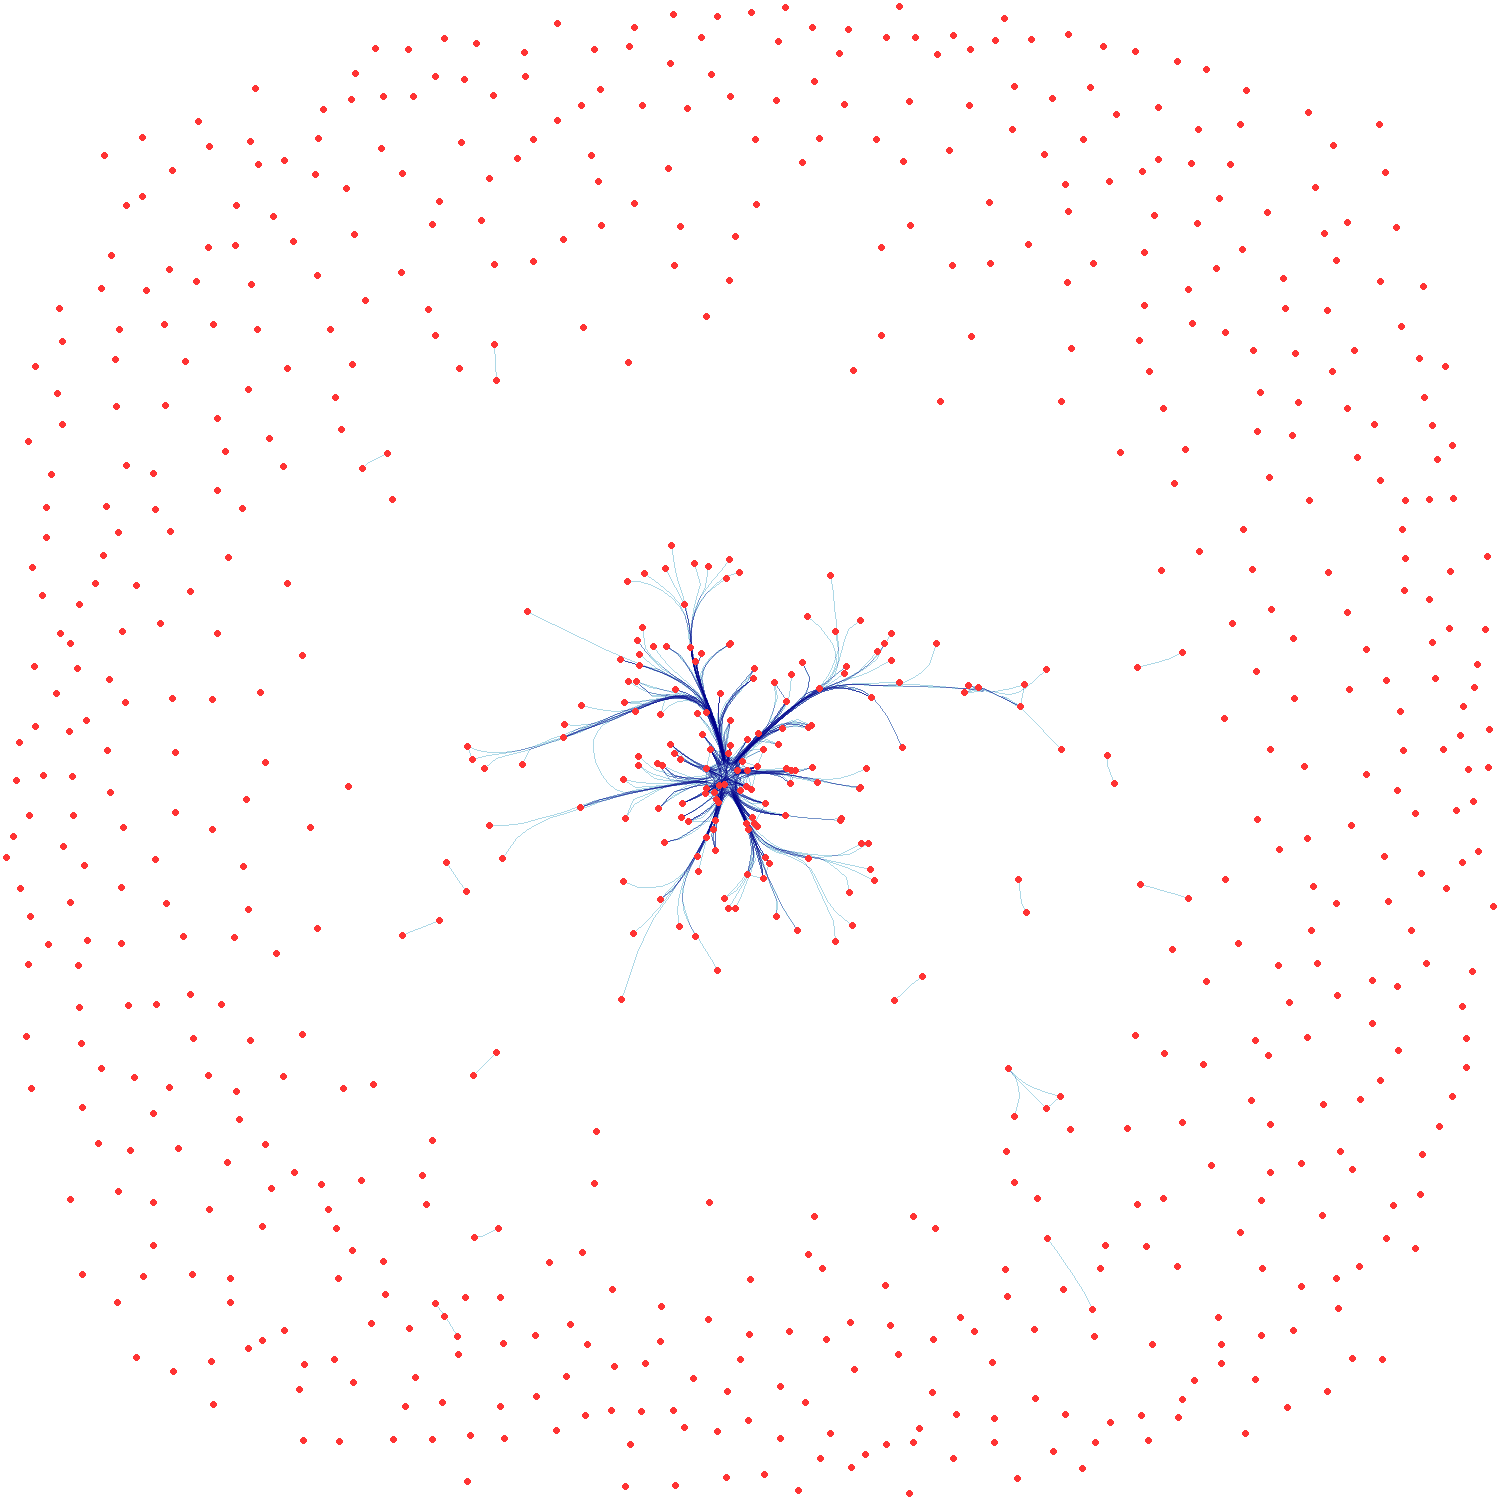
\includegraphics[width=.25\textwidth]{/files/src/.media/ego/grafo_forceatlas2_8.png}}\hfill
    \subfloat[$u = 9$]{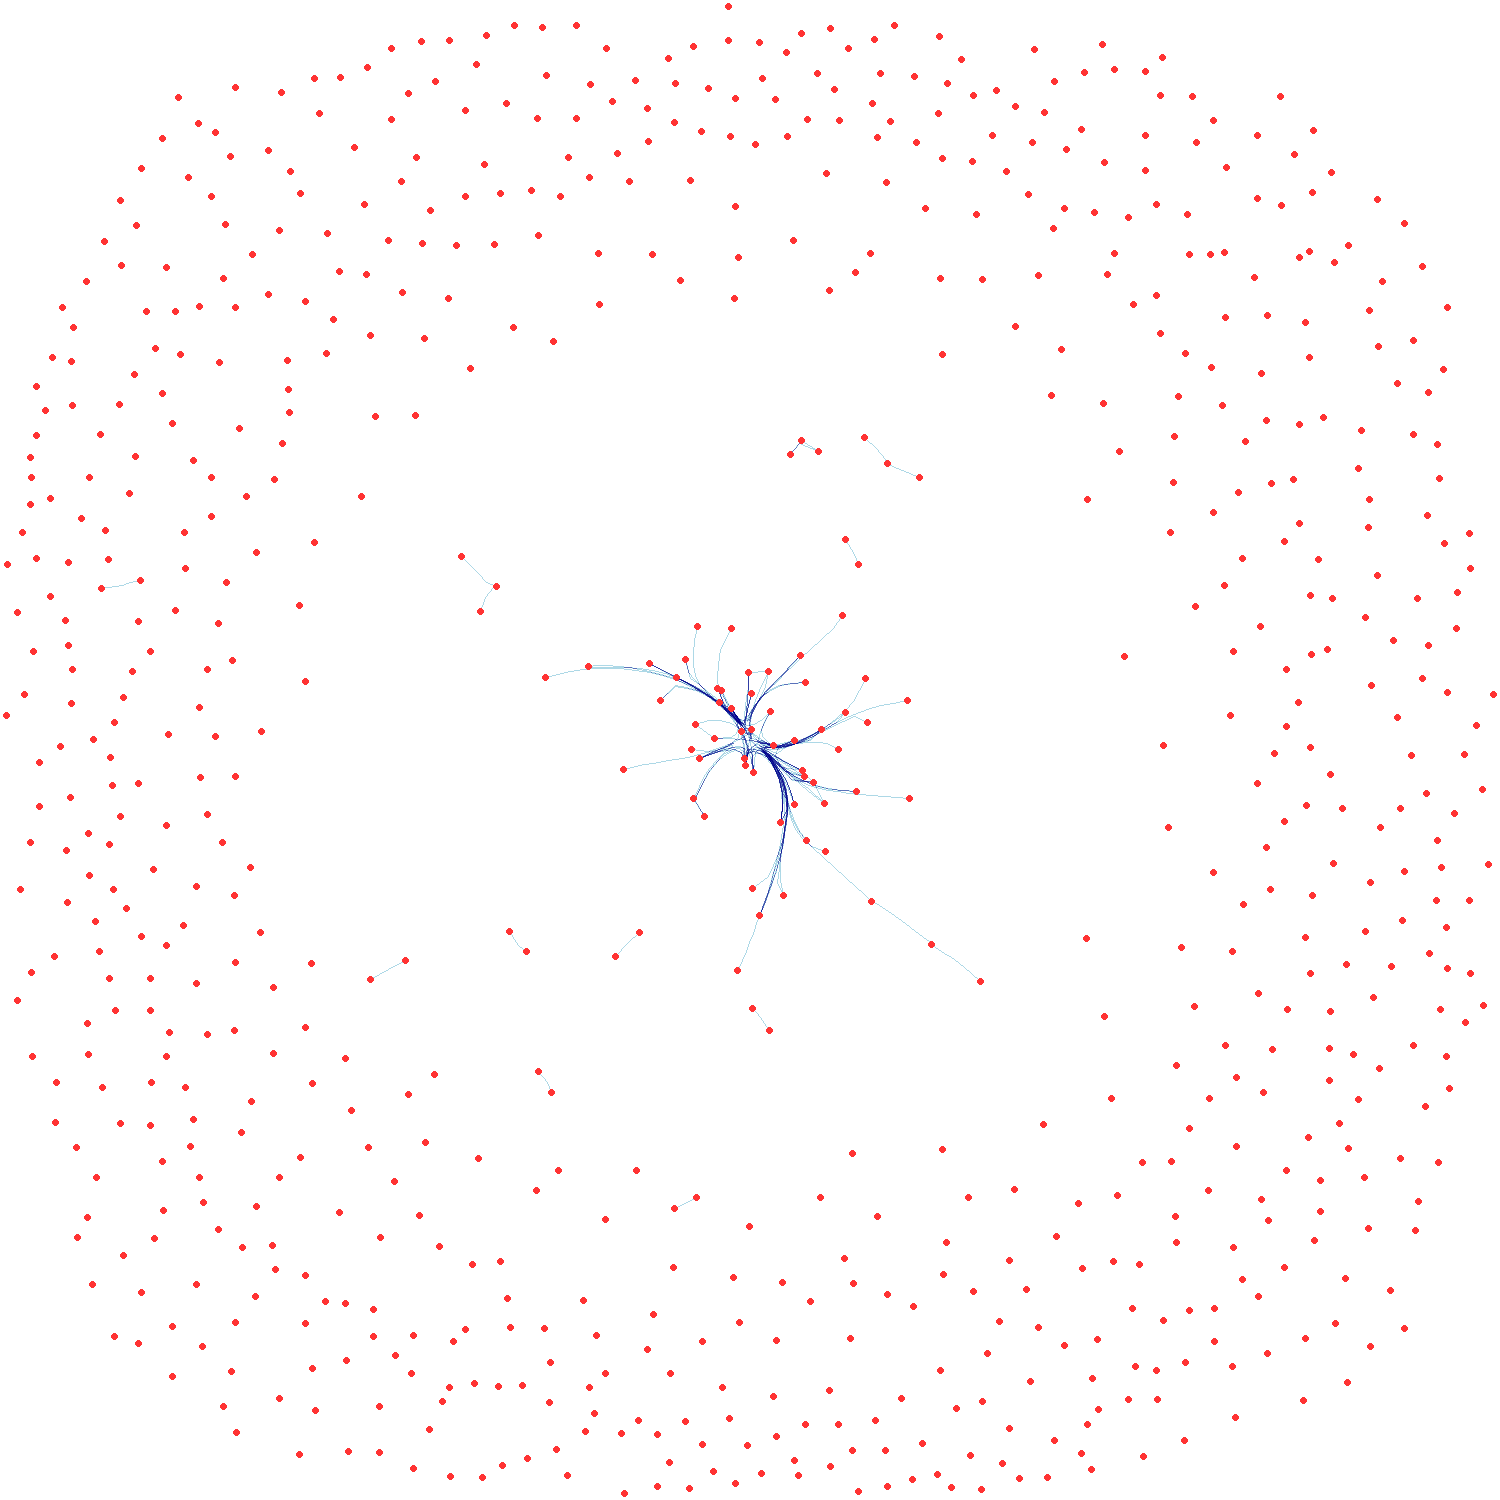
\includegraphics[width=.25\textwidth]{/files/src/.media/ego/grafo_forceatlas2_9.png}}\hfill
    \subfloat[$u = 10$]{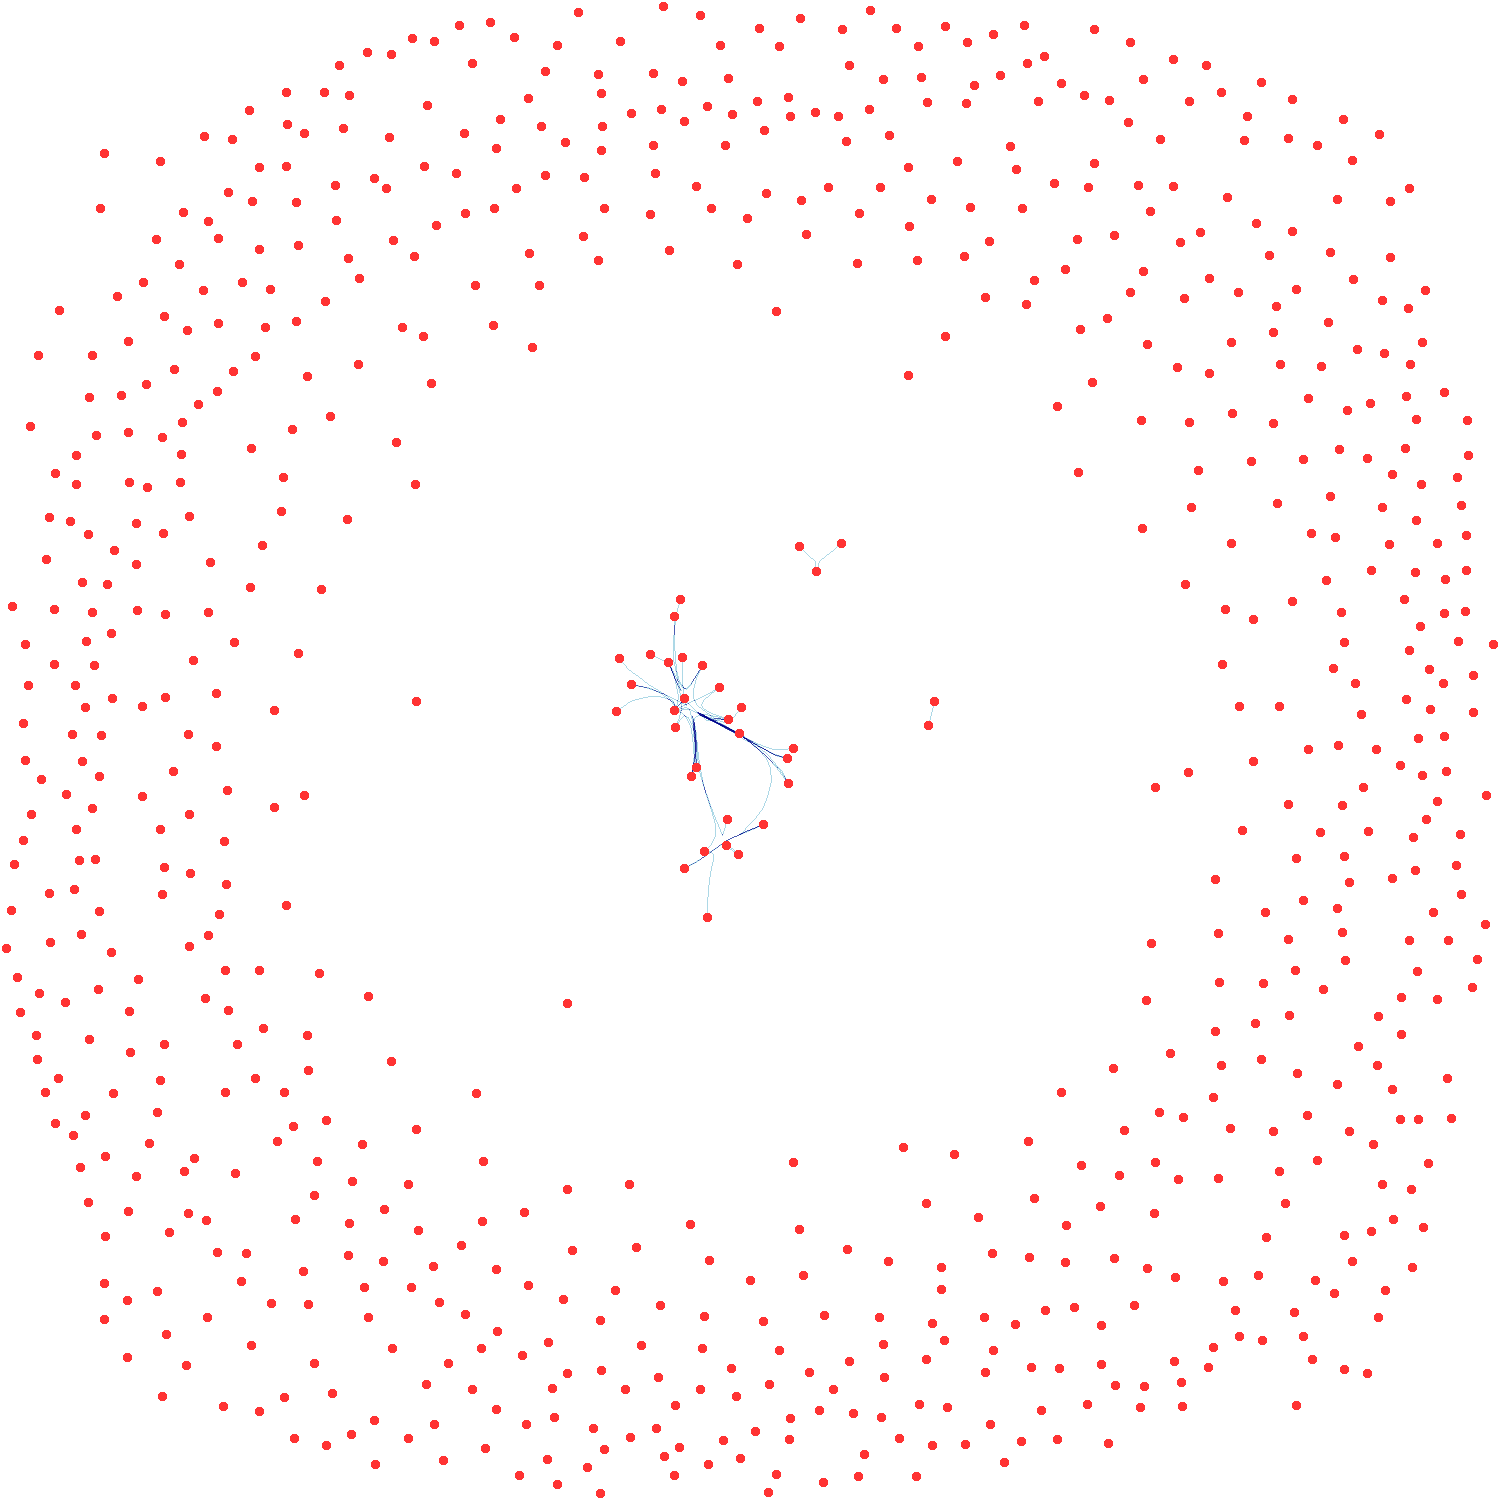
\includegraphics[width=.25\textwidth]{/files/src/.media/ego/grafo_forceatlas2_10.png}}\hfill
    \\[\smallskipamount]
    \subfloat[$u = 11$]{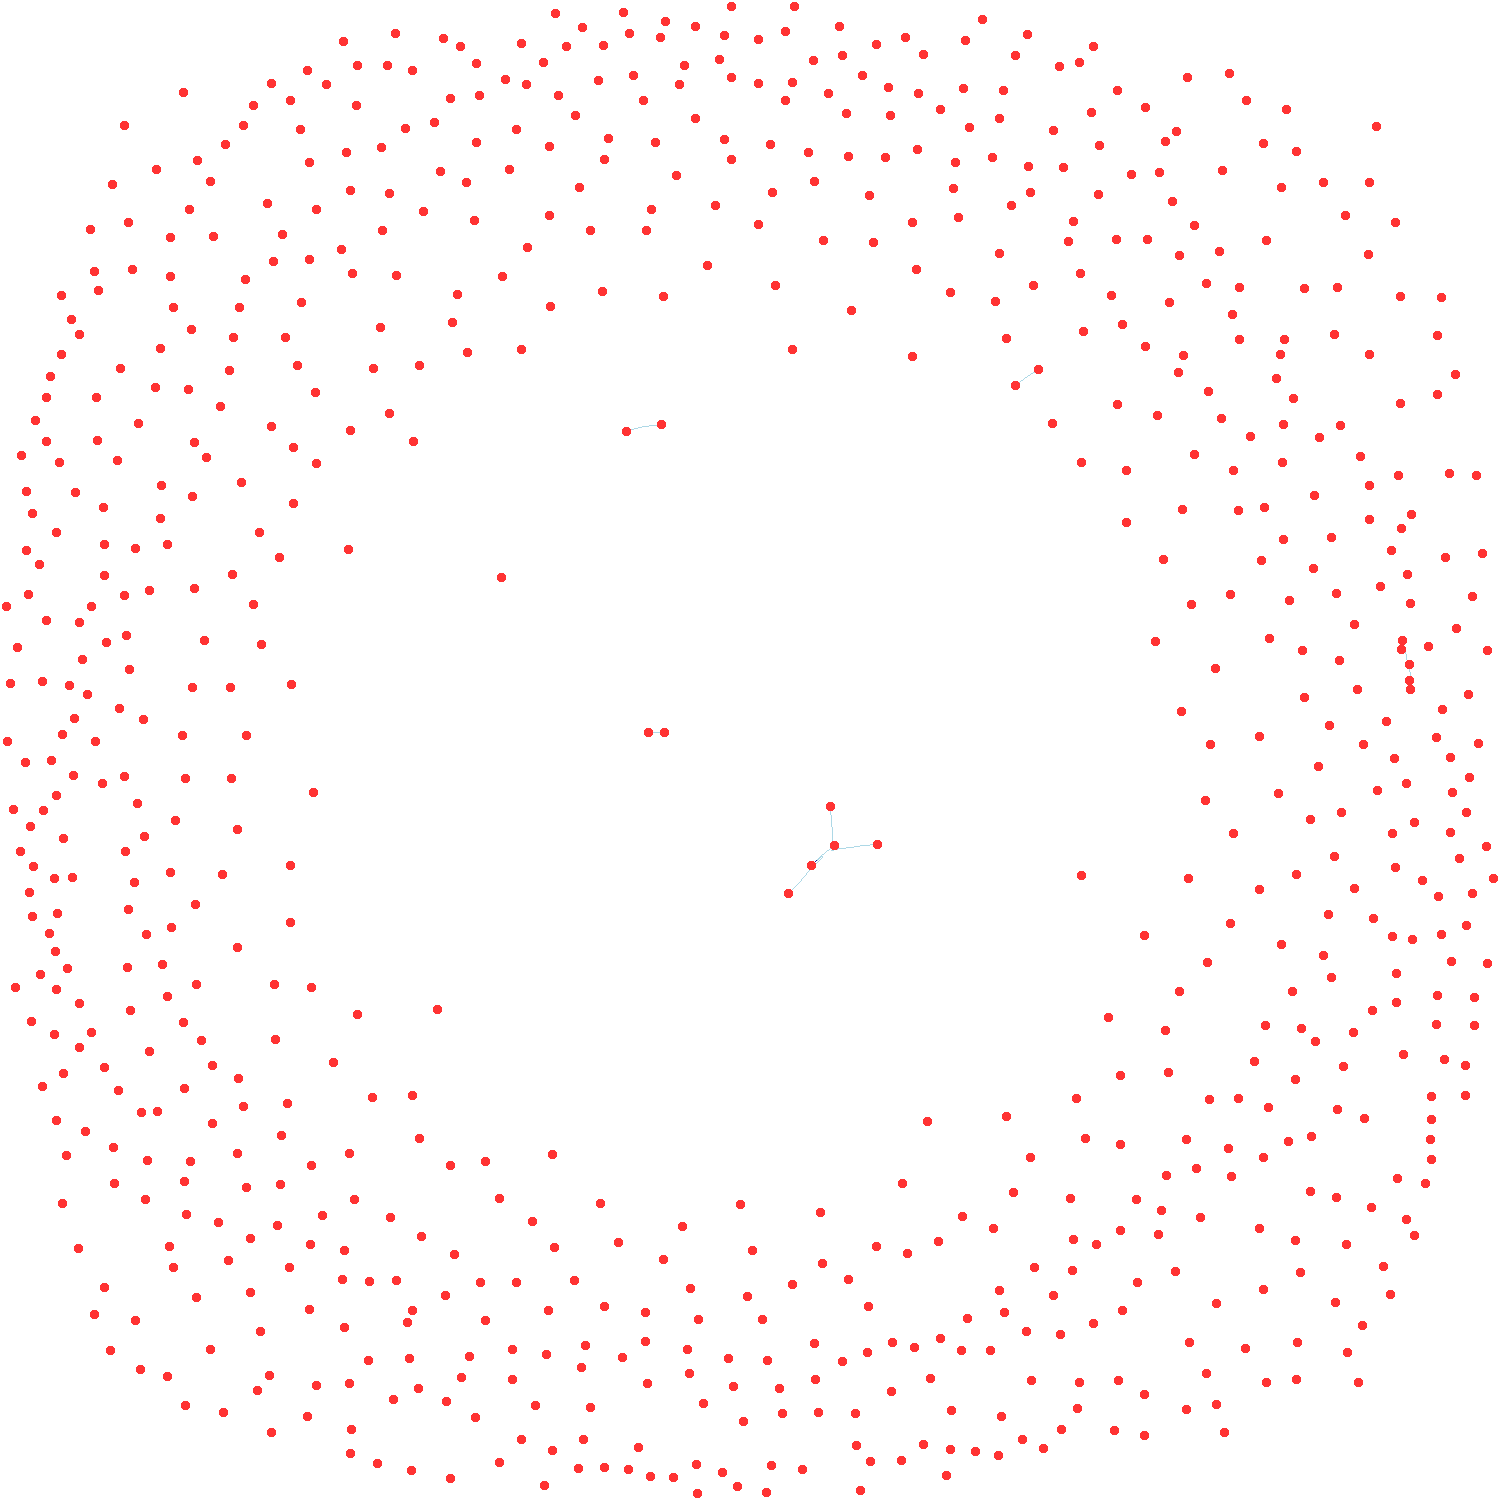
\includegraphics[width=.25\textwidth]{/files/src/.media/ego/grafo_forceatlas2_11.png}}\hfill
    \subfloat[$u = 12$]{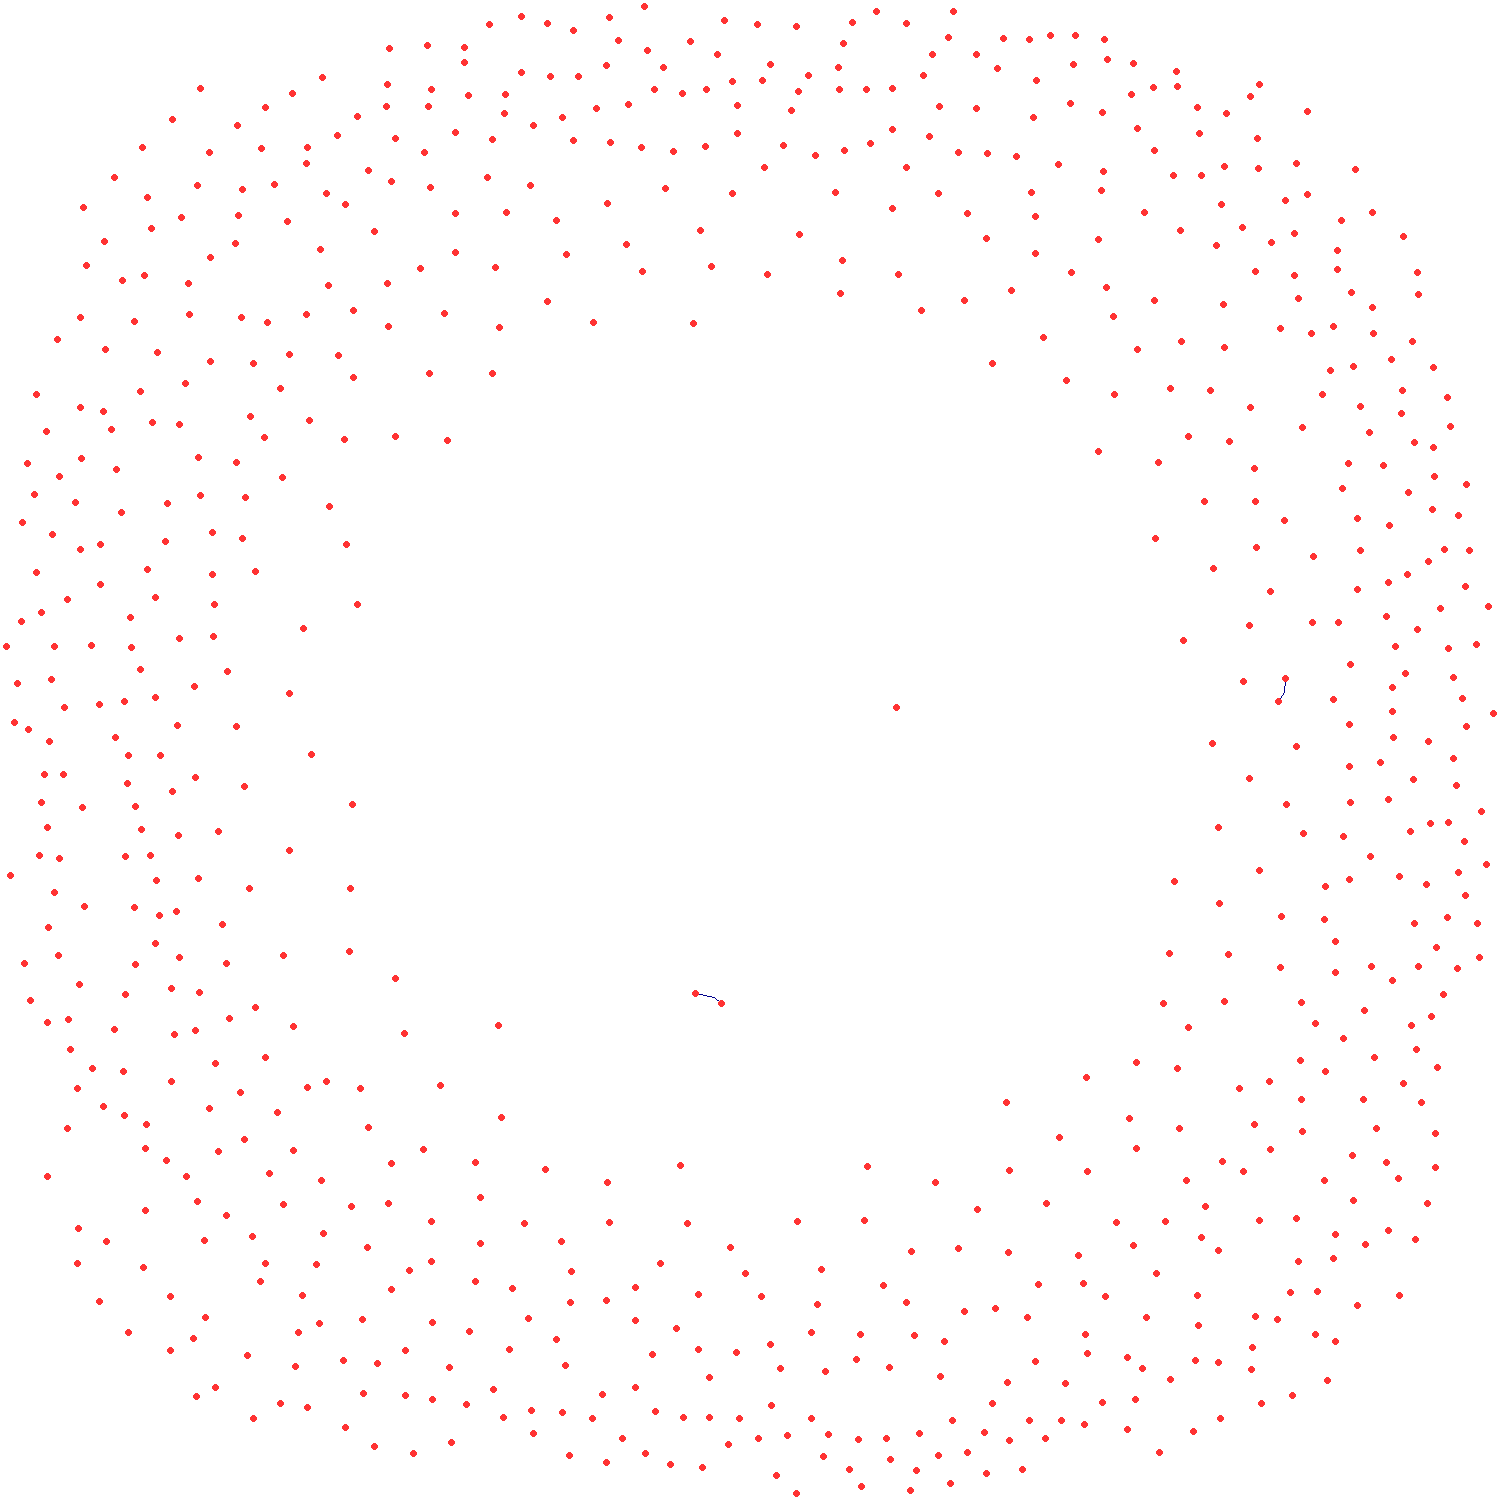
\includegraphics[width=.25\textwidth]{/files/src/.media/ego/grafo_forceatlas2_12.png}}\hfill
    \caption{Todos los grafos correspondientes a los diferentes umbrales, tomados para la matriz de similaridad de los atributos \textbf{C}. Observar que al aumentar $u$ crece la cantidad de nodos aislados.}
\end{figure}

\vspace{1em}


% === COMPARACION === %

\vspace{2em}
\subsection{Comparación con la red original}

Nos encontramos con diferentes grafos construidos en base a los atributos en \textbf{C}. Buscamos ahora comparar nuestras aproximaciones con la red original. 
Un primer acercamiento a este problema fue calcular la cantidad de posiciones coincidentes entre las matrices de adyacencia y dividir por los elementos totales. La lógica por detrás del método es que nuestros grafos serán más similares entre sí por cada conexión y `no conexión' acertada. Entonces, por cada 0 y 1 coincidente en nuestra aproximación y \textbf{E} nos acercaríamos más a un 100\% de similitud. 

\begin{figure}[!htbp]
\begin{equation*}
    \begin{bmatrix}
    0  &\%\ 7.6054231   \\
    1  &\%\ 32.947445   \\
    2  &\%\ 58.570142   \\
    3  &\%\ 70.993985   \\
    4  &\%\ 84.162733   \\
    5  &\%\ 91.537012   \\
    6  &\%\ 94.322073   \\
    7  &\%\ 95.214277   \\
    8  &\%\ 95.403337   \\
    9  &\%\ 95.446393   \\
    10 &\%\ 95.455457   \\
    11 &\%\ 95.458695   \\  
    12 &\%\ 95.459342   \\
    13 &\%\ 95.459990   \\
    \end{bmatrix}
\end{equation*}
\caption{Similitud elemento a elemento de las matrices de adyacencia, la primer columna representa el umbral tomado para la aproximación y la segunda el porcentaje de elementos correctamente estimados con respecto a la original. Se incluye un grafo sin aristas, con $u = 13$.} \label{promedio_similaridad}
\end{figure}

Como puede observarse, desafortunadamente, los grafos con muy pocas conexiones, como prueban ser tomando los umbrales $u > 10$, tienen de los valores más altos, mientras que otros con cantidad de aristas similares a la red original, como con $u = 5$ o $u = 6$ (16.850 y 5.727 conexiones respectivamente), parecerían ser peores aproximaciones. Esto se da por la naturaleza rala de nuestras matrices de adyacencia. La de la red `ego' \textbf{E} es de $786 \times 786$, con 617.796 elementos, y tan solo 28.048 (\% 4.54) de ellos son no nulos. Es decir, es rala en un \% 95.46. Es por esto que comparar elemento a elemento no prueba ser un método muy descriptivo de qué tan buena es una aproximación, ya que cualquiera con pocos elementos coincidirá en un $\sim$\% 95.

\vspace{1em}

Empleamos entonces otros dos métodos de comparación: \textit{la correlación de las matrices de adyacencia estiradas} y \textit{la correlación de las listas de autovalores}. La correlación es una covarianza normalizada con valores en (-1, 1), donde números mayores indican una mayor similitud. Esta es descrita por la siguiente fórmula:

\begin{equation}
    Corr(x, y) = \frac{(x - \mu_{x}) \cdot (y - \mu_{y})}{\sqrt[]{(x - \mu_{x})^{2} \cdot (y - \mu_{y})^{2}}}
\end{equation}

siendo $\mu$ el valor medio de los vectores.

\vspace{1em}
\begin{figure}[!htbp]
\centering
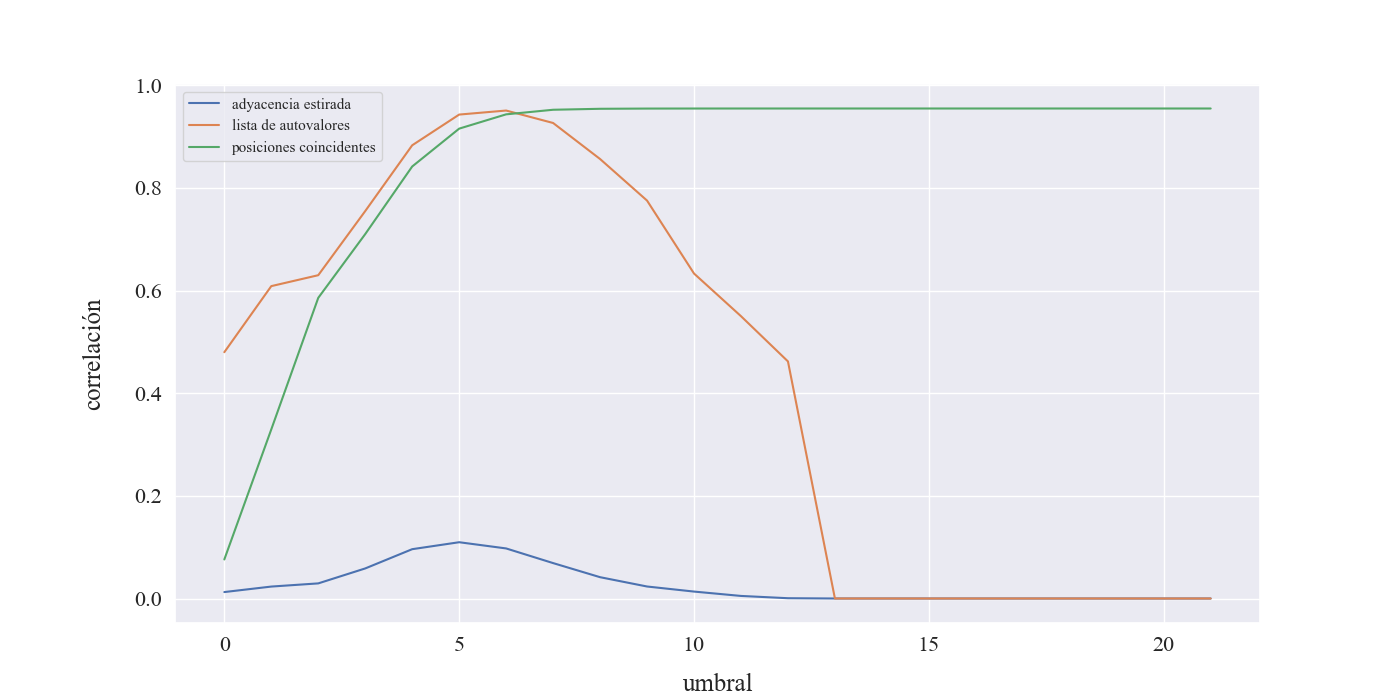
\includegraphics[scale=0.45]{/files/src/.media/ego/facebook_similaridad.png}
\caption{Correlaciones entre matrices de adyacencia y listas de autovalores según los diferentes umbrales.}
\label{grafo_correlaciones}
\end{figure}

En la figura (\ref{grafo_correlaciones}.) se puede apreciar que se obtienen resultados considerablemente diferentes a los de nuestro primer método de comparación. En un primer lugar, siguiéndonos de la correlación entre las matrices de adyacencia, parecería que las mejores aproximaciones son las de cantidad de aristas similares a la red original, con los umbrales $u \in [4,7]$, mientras que los grafos vacíos con umbrales más altos pasan a tener correlación 0. De la misma forma, analizando con los autovalores se obtienen resultados similares, donde la mayor correlación se halla con los umbrales de valores medios.  


% === OPTIMIZACION === %

\vspace{2em}
\subsection{Optimización}




% === PCA === %

\vspace{2em}
\subsection{PCA}
